Ce chapitre détaille le développement des différents aspects du SG. Une vision globale de l'ensemble du SG, est disponible dans le chapitre "Résultats", à la section \ref{sResActualSG}.  Premièrement, afin d'avoir une vue d'ensemble, sa structure est détaillée sous plusieurs aspects dans la section \ref{sDevStructure}. Ceci afin d'avoir une idée sur la façon dont le projet est exécuté, construit et implémenté. Ensuite, les détails sur l'implémentation des principales fonctionnalités du SG (d'après les objectifs) sont décrits en trois autres sous-sections. La section \ref{sDevAppauvrissement}, décrit en détail le système d'appauvrissement actuel mais également tous les tests ayant été réalisés pour y arriver. La section \ref{sDevDeroulementPartie} décrit différents éléments liées à l'aspect "jeu" du SG et décrit également le déroulement d'une partie. La dernière, section \ref{sDevArticulation}, parle de la présence des différents mouvements de marche dans le SG et de l'articulation de l'avatar.
\\

Sur la fin du développement, Monsieur Kevin Laipe, un stagiaire du groupe imagerie de la HE-Arc a été mis à contribution pour ce projet. Sous ma supervision, il a réalisé principalement des tâches de design pour enrichir quantitativement le SG. Sur la fin, le développement de certaines fonctionnalités lui ont été assignées. Son aide a permis d'étoffer le contenu du SG, d'identifier les différents \textit{bugs} grâce à de nombreux tests et de tester l'architecture du SG. L'ajout de niveaux et fonctionnalités a permis de tester le faible couplage des fonctionnalités existantes et la facilité d'ajout de contenu. Les éléments réalisés par Monsieur K. Laipe sont les mondes supplémentaires (de deux à cinq), l'appauvrissement des animations, l'ajout du son de scintillement aux objectifs, la scène utilitaire "ObjectiveViewGenerator" et les images des objectifs utilisées dans le choix des niveaux.%TODO: Éviter la formulation "MON encadrement"

\section{Structure du projet}
	\label{sDevStructure}
	Dans cette section est décrite, sous plusieurs aspects, la structure du projet. La langue choisie pour nommer les différents éléments développés est l'anglais. Les exemples de cette section ont donc des noms anglais.
	\subsection*{Structure du projet et environnement}
	La communication et les différentes entités nécessaires à l'exécution du projet sont implémentées comme elles ont été conçues (section \ref{sConCommunication}). Comme dans le précédent projet, le programme tiers faisant le lien entre Ocf et la mémoire partagée met constamment à jour ses valeurs afin de garantir le temps réel. Trois projets C\# \cite{CSharp_website} ont été réalisés pour implémenter cette communication:
	\begin{itemize}
		\item \textbf{ClientSharedMemoryLibrary --} Ce projet crée une libraire "ClientSharedMemoryLibrary.dll" en \textit{.NET} 3.5 pour pouvoir utiliser la mémoire partagée. Bien que Unity supporte officiellement \textit{.NET} 2.0, certains aspects de la version 3.5 sont utilisables (tels que la mémoire partagée) \cite{UnityDotNETVersion};
		\item \textbf{ServerSharedMemoryProcess --} Ce projet crée un exécutable en \textit{.NET} 4.5 (pour l'utilisation de types dynamiques). Celui-ci récupère, à son lancement, les paramètres initiaux (l'inclinaison du siège). Puis, en boucle, dans un \textit{thread} séparé, les dernières valeurs de l'application temps réel à l'aide d'Ocf. Il les place ensuite dans la mémoire partagée pour être accessible au client;
		\item \textbf{SGData --} Ce projet crée une librairie "SGData.dll" \textit{.NET} 3.5 contenant toutes les classes passées dans la mémoire partagée.
	\end{itemize}
	Le client de la mémoire partagée peut réaliser trois actions: demander les paramètres initiaux; demander les dernières valeurs; fermer la mémoire partagée. C'est quand il demande les dernières valeurs qu'il indique si le jeu est terminé ou non. Cette information est ensuite transmise à l'application temps réel qui termine l'exercice. L'exercice peut également être terminé par le thérapeute, depuis l'IHM. Dans ce cas, le SG le saura en récupérant les dernières valeurs (l'état du LHS sera "StopExerciseState", voir section \ref{sConCommunication}).	
	%TODO: Parler d'un ordre de lancement
	
	La persistance du projet se fait actuellement en local sur l'ordinateur exécutant les SG. Seul un fichier, nommé "save.dat" est créé et il se trouve dans le dossier "\%AppData\%/LocalLow/HEArc/SGTM". Le SG ne tient pas compte de plusieurs utilisateurs. La principale raison étant que l'identification du patient n'est pas possible à l'aide des variables mises à disposition par l'application temps réel. Ce fichier binaire contient pour chaque niveau, un ensemble de numéros représentant les objectifs (traces de civilisation) déjà obtenus. Afin de réinitialiser les sauvegardes du SG, il suffit de supprimer ce fichier.
	\subsection*{Structure des \textit{Assets}}
		Parmi les sous-répertoires du projet \textit{Unity}, seul le contenu du dossier "Assets" a été modifié manuellement et est décrit dans ce rapport. Il contient toutes les ressources nécessaires au SG (figure \ref{structProjet}).\medskip
		
		\begin{minipage}{\linewidth}
			\makebox[\linewidth]{
				\includegraphics[]{img/Developpement_AssetHierarchy.PNG}}
			\captionof{figure}{Contenu du répertoire "Assets".}
			\label{structProjet}
		\end{minipage}\medskip
		
		Voici une description de leurs contenus:
		\begin{itemize}
			\item \textbf{Animations --} Ce répertoire contient tous les objets \textit{Animator} et \textit{Animations} créés dans ce projet. Les animateurs sont nommés "XAnimator" et les animation "XY" où X est le type d'objet à animer (\textit{e.g.}, "Gate") et Y est l'action réalisée (\textit{e.g.}, "Open"). Si le contrôleur ne contient qu'une animation, celle-ci se nomme "XAnimation". Toutes les animations ne sont pas présentes dans ce dossier. Celles provenant de sources trouvées sur internet (\textit{e.g.}, les animations de marche) se trouvent dans des sous-dossiers du dossier "\textit{Plugins}" décrit plus bas dans cette liste;
			\item \textbf{ Fonts --} Ce répertoire contient les polices de caractères utilisées dans ce projet;
			\item \textbf{ Materials --} Ce répertoire contient tous les objets \textit{Material} créés ou modifiés dans ce projet. Tous les matériaux du SG ne sont pas présents dans ce répertoire. Les matériaux créés automatiquement durant l'importation d'objets 3D sont présents dans le répertoire de destination de cette importation. Celui-ci étant un sous-répertoire de "Meshes" décrit plus bas dans cette liste; 
			\item \textbf{Meshes --} C'est dans ce répertoire que tous les modèles 3D (tel que \textit{.obj} ou \textit{.fbx}) trouvés sur internet sont importés. Chaque modèle est importé dans son propre sous-répertoire et certains sont regroupés en famille dans d'autres. L'importation crée de nombreuses ressources textures ou \textit{Material}. Celles-ci ne sont pas déplacées dans les répertoire "Textures" ou "Materials" mais laissées dans le sous-répertoire de l'importation.
			\begin{itemize}
				\item \textbf{Avatar --} Ce répertoire contient quatre sous-répertoires. Deux pour la tête et le costume d'un avatar féminin et deux pour ceux masculin. Dans le SG, seul le modèle féminin est utilisé actuellement. Si l'indication du sexe du patient peut être communiquée au SG, il est possible de lui choisir un avatar adapté;
				\item \textbf{Decorations --} Ce répertoire contient les différents modèles 3D utilisés en décoration dans les mondes (\textit{e.g.}, planètes, cascade, etc.). Ce sont des objets placés dans les mondes manuellement et ne subissant pas d'appauvrissement géométrique ou quantitatif;
				\item \textbf{Interior --} Ce répertoire contient les différents modèles 3D utilisés pour créer l'intérieur du vaisseau spatial (zone familière);
				\item \textbf{Landscape Elements --} Ce répertoire contient les différents modèles 3D utilisés pour créer les "\textit{Landscape elements}". Ce sont les objets placés massivement par script dans la scène dont la géométrie et la quantité peuvent être appauvries. Les modèles 3D de ce répertoire corresponde à leur modélisation totale ("\textit{FullGeometry}, voir section \ref{sDevAppauvrissement});			
				\item \textbf{Objectives --} Ce répertoire contient les différents modèles 3D utilisés pour les objectifs placés dans la scène;			
				\item \textbf{Spaceship --} Ce répertoire contient les différents modèles 3D du vaisseau spatial.	
			\end{itemize}
			\item \textbf{Plugin --} Ce répertoire contient les différents modules d'extension, les packs de ressources trouvés sur l'\textit{Assets store} \cite{UnityAssetStore_website} de \textit{Unity} ou encore les librairies (\textit{.dll}) utilisées par le SG.
			\begin{itemize}
				\item \textbf{Oculus --} Module d'extension pour l'utilisation de l'\textit{Oculus Rift} \cite{OculusDk2_website}. Depuis la version 5.1 \cite{UnityOculusIntegration}, \textit{Unity} ne nécessite plus de \textit{plugin} pour fonctionner avec ce HMD. Cependant, le résultat obtenu était perceptiblement plus saccadé que lors de l'utilisation du \textit{plugin}, c'est pourquoi il est encore utilisé dans ce travail. Ce phénomène a été constaté visuellement et aucune mesure n'a été faite. Sa source ou sa possible reproduction dans d'autres situations est inconnue. Ce n'est donc qu'une expérience vécue et non un fait avéré; %TOO: Jugement de valeur, à faire valider par STG
				\item \textbf{Raw Mocap Data --} Ce paquet est mis à disposition gratuitement par \textit{Unity}. Il contient différentes animations de marche, course, saut, etc. pour animer un avatar humanoïde. C'est de ce paquet que vient l'animation de marche du guide;
				\item \textbf{SG\_LHS --} Ce répertoire contient les deux librairies utiles à la communication avec le LHS. Celles-ci sont détaillés dans la sous-section précédente;
				\item \textbf{Standard Assets --} Ce paquet est mis à disposition gratuitement par \textit{Unity}. Il contient un certain nombre d'effets implémentés dans des scripts et des \textit{shaders}. Il est utilisé pour l'effet de flou de mouvement lors d'une téléportation.
			\end{itemize}
			\item \textbf{Prefabs, Scenes, Scripts --} Ces répertoires contiennent respectivement les \textit{Prefabs}, scènes et scripts. Chacun d'entre eux a une structure et une importance plus grande que les autres répertoires décrits dans cette sous-section. C'est pourquoi, une sous-section entière est dédiée à chacun d'eux, plus bas dans ce document;
			\item \textbf{Shaders --} Ce répertoire contient les différents \textit{shaders} écrits pour le SG;
			\item \textbf{Skyboxes --} Ce répertoire contient les différentes \textit{skyboxes} utilisées dans les différents mondes. Elles ont été trouvées sur internet;
			\item \textbf{Sounds --} Ce répertoire contient un sous-répertoire pour chaque type de son (détaillés dans la section \ref{sDevAppauvrissement});
			\item \textbf{Terrains --} Ce répertoire contient un sous-répertoire pour chaque niveau. Ceux-ci contiennent:
			\begin{itemize}
				\item Une image représentant le monde (utilisée dans le choix des niveaux);
				\item Trois fichiers de terrains, étant les trois niveaux d'appauvrissement de sa géométrie (voir section \ref{sDevAppauvrissement});
				\item Une "\textit{LandscapeElementsMap}", étant une image permettant la génération des "\textit{Landscape elements}" (voir \ref{sDevDeroulementPartie});
				\item Un fichier XML décrivant le chemin. Celui-ci décrit le chemin qui est imposé à l'utilisateur pour ce niveau. Plus de détails sur sa création et son utilisation dans la section \ref{sDevDeroulementPartie}.
			\end{itemize}
			
			\item \textbf{Textures --} Ce répertoire contient les textures créées ou manuellement assignées aux objets du SG. Les textures issues de l'importation de modèles 3D ou générée par scripts se trouvent, quant à elles, dans les répertoires de destination de ces importations ou générations. Les textures utilisées pour l'interface graphique ou le HUD sont, elles, importées en tant que \textit{sprites} et présentes dans le sous-répertoire "UI". Ce sous-répertoire contient également les fichiers de dessin de ces différents boutons ou icônes. Ces fichier ".svg" sont réalisés avec le logiciel \textit{Inkscape}, un logiciel libre de dessin vectoriel \cite{Inkscape_website}. Le sous-répertoire "Ground" contient toutes les textures utilisées sur les terrains. Le sous-répertoire "RenderTextures" contient toutes les \textit{RenderTextures} utilisées dans ce travail. Ces dernières permettent d'afficher en tant que texture ce que voit une caméra. D'autres textures sont directement contenues dans ce répertoire. C'est le cas de celles placées directement dans les scènes en décoration. La texture "\textit{Space Traveling in the speed of light - Royalty Free Footage}" a la particularité d'être une texture animée (vidéo). Elle nécessite d'avoir \textit{Quicktime} \cite{QuickTime_website} installé pour être importée correctement \cite{UnityMovieTexture}.
			%TODO: Faire une section Prérequis ?
		\end{itemize}	
		
	\subsection*{Structure des \textit{Prefabs}}
		Les \textit{Prefabs} sont des \textit{GameObject} (éléments composant les scènes) dont la configuration est enregistrée. Ceux-ci peuvent être utilisés dans plusieurs scènes et y être instanciés dynamiquement. Une modification sur un objet préfabriqué, l'applique à chacune de ses utilisations. Il est recommandé, même si un objet est utilisé dans une seule scène \cite{Unity50Tips} d'en créer un objet préfabriqué. Cela minimise les changements sur la scène et facilite la résolution de conflits, si on utilise un serveur de versionnement. Dans ce travail, de nombreux objets préfabriqués ont été créés. Ceux-ci se trouvent dans le répertoire "Prefabs" (figure \ref{structPrefabs}).\medskip
		
		\begin{minipage}{\linewidth}
			\makebox[\linewidth]{
				\includegraphics[]{img/Developpement_StructurePrefabs.PNG}}
			\captionof{figure}{Contenu du répertoire "Prefabs".}
			\label{structPrefabs}
		\end{minipage}\medskip
		
		Ce répertoire contient quelques objets préfabriqués ainsi que des sous-répertoires. Premièrement, voici une liste des objets préfabriqués qu'il contient:
		\begin{itemize}
			\item \textbf{ComputationalAvatar --} Cet objet est chargé si on utilise en entrée le clavier (quand le SG n'arrive pas à se connecter au LHS). Il contient un avatar invisible sur lequel est effectué une animation de marche lorsque l'on avance (flèche haut ou touche "w"). L'angle des articulations est ensuite relevé, par le script gérant les entrée/sorties, puis transmis à l'avatar principal pour l'animer en fonction;
			\item \textbf{Controllers --} Cet objet préfabriqué est contenu dans chaque niveau et contient tous les scripts contrôleurs utiles au déroulement d'une partie \cite{UnityMVC} (structure des scripts expliquée dans la section suivante);
			\item \textbf{EnterSceneAnimator --} Cet objet préfabriqué est contenu dans tous les mondes et l'animation d'atterrissage en début de niveau;
			\item \textbf{Guide --} Cet objet préfabriqué contient le guide et est présent dès la scène de sélection du niveau (structure des scènes expliquée dans une autre sous-section);
			\item \textbf{ImpoverishmentControllers --} Cet objet préfabriqué contient tous les scripts contrôleurs de l'appauvrissement. Il est présent dès la scène de sélection des niveaux;
			\item \textbf{Models --} Cet objet préfabriqué est présent dans la scène de sélection des niveaux. Il contient les différents modèles \cite{UnityMVC} nécessaires au fonctionnement du SG;
			\item \textbf{Objective --} Cet objet est à ajouter à chaque objet 3D représentant un objectif dans les scènes de jeu. Une fois placé et configuré (voir section \ref{sDevDeroulementPartie}), il les rend disponible au \textit{scan} et permet leur placement sur la gauche ou sur la droite du chemin.
			\item \textbf{ObjectiveMiniMapView --} Cet objet préfabriqué est instancié dynamiquement dans les niveaux. Il représente la zone où un objectif est présent sur la carte;
			\item \textbf{PlayerFemale, PlayerMale --} Ces objets préfabriqués sont, respectivement, l'avatar homme et femme. Le SG ne pouvant pas récupérer l'information du sexe du patient, seul l'avatar femme est utilisé pour le moment. Il est présent dès la scène de sélection des niveaux;
			\item \textbf{SpaceshipWithInterior --} Cet objet préfabriqué contient le vaisseau et ses pièces intérieures. Il est présent dès la scène de sélection des niveaux;
			\item \textbf{TeleportationRings --} Cet objet est instancié dynamiquement, si le temps dans un niveau est écoulé. Il contient les anneaux de téléportation se plaçant autour du joueur.
		\end{itemize}
		
		Deuxièmement, voici une description des sous-répertoires:
		\begin{itemize}
			\item \textbf{Interior --} Ce sous-répertoire contient les objets préfabriqués utilisés pour meubler l'intérieur du vaisseau spatial. Ce sont les objets qui sont considérés comme des éléments familiers;
			\item \textbf{Landscape elements --} Ce sous-répertoire contient un répertoire pour chaque type de géométrie des \textit{landscape elments}. Ceux-ci contiennent chacun un objet préfabriqué ou un autre répertoire pour chaque type ou famille de \textit{landscape elments}. Les \textit{landscape elments} étant les objets placés par script sur le terrain dont la géométrie et la quantité peuvent être appauvries (voir section \ref{sDevAppauvrissement}). Il contient également un sous-répertoire "Referencer". Celui-ci contient les \textit{landscape elments} référençant chacune de leur géométrie;
			\item \textbf{UI --} Ce sous-répertoire contient les objets préfabriqués utilisés dans l'interface de sélection des niveaux. Il contient un répertoire "ObjectiveViews" contenant les aperçus de tous les objectifs;
			\item \textbf{Worlds --} Ce sous-répertoire en contient un pour chaque niveau. Chacun contient les objets préfabriqués propres à chaque niveau. Voici une description de leur contenu:
			\begin{itemize}
				\item \textbf{Decorations --} Répertoire non obligatoire. Contient toutes les décorations utilisées dans le monde. Une décoration étant un objet n'ayant aucune interaction ni appauvrissement géométrique et quantitatif;
				\item \textbf{Landscape elements Families --} Répertoire obligatoire. Contient les différentes familles de \textit{landscape elments} utilisées dans le niveau;
				\item \textbf{Objectives --} Répertoire obligatoire. Contient tous les objectifs configurés du niveau;
				\item \textbf{GroundTerrain --} Objet préfabriqué obligatoire. Référence les bruits de pas pour chaque type de sol (voir section \ref{sDevAppauvrissement});
				\item \textbf{LevelX --} Objet préfabriqué obligatoire. Référence les différents éléments de visualisation du niveau (pour la sélection), ainsi que les éléments nécessaires au chargement de celui-ci.
			\end{itemize}
			
			Ce répertoire contient également un objet préfabriqué nommé "\textit{TerrainElements}". Il doit être placé dans toutes nouvelles scènes en tant qu'enfant de l'objet "Terrain". Il contient les principaux éléments d'un Terrain: La caméra affichant la mini-map, les lumières et la source audio de la musique de fond.
		\end{itemize}
	
	\subsection*{Structure des scripts}
		La structure des scripts suit le patron d'architecture modèle-vue-contrôleur (MVC) \cite{UnityMVC}, présenté dans la figure \ref{structScripts}. De façon générale, elle veille à minimiser l'interdépendance des script, afin de faciliter l'ajout ou la suppression d'une fonction.\medskip
		
		\begin{minipage}{\linewidth}
			\makebox[\linewidth]{
				\includegraphics[]{img/Developpement_StructureScripts.PNG}}
			\captionof{figure}{Contenu du répertoire "Prefabs".}
			\label{structScripts}
		\end{minipage}\medskip
		
		Le dossier contient deux scripts: "\textit{SGMonoBehaviour}" et "\textit{InGameUpdatableSGMonoBehaviour}", dont la structure est schématisée dans un diagramme UML, en annexe. Le premier dérive de la classe "\textit{MonoBehaviour}". Cette classe \textit{Unity} est celle qu'un script doit hériter s'il veut être accroché dans la scène à un \textit{GameObject}. La classe "\textit{SGMonoBehaviour}" implémente des méthodes supplémentaires permettant de récupérer les objets de la scène implémentant une interface. La classe \textit{GameObject} propose de telles méthodes mais qui ne fonctionnent qu'avec les classes héritant de \textit{UnityEngine.Object}. Ces fonctions ont été trouvées sur un article proposant des bonnes pratiques pour le développement \textit{Unity} \cite{Unity50Tips}. Tous les scripts de ce travail devant être accroché à un \textit{GameObject} héritent donc de \textit{SGMonoBehaviour} (ou d'une classe enfant).
		\\
		
		La deuxième de ces classes est dérivée par tous les scripts devant être mise à jour à chaque moment d'un niveau du SG. Elle permet de définir un comportement pour les états de pause et de fin de jeu, ainsi que d'implémenter une logique d'activation ou de désactivation. Elle offre également une référence directe à la classe \textit{GameController}. Pour cela, il faut utiliser les méthodes "\textit{\_Start()}" et "\textit{\_Update}" au lieu de "\textit{Start()}" et "\textit{Update}".
		\\
		
		Quatre sous-répertoires sont ensuite présents: "\textit{Model}", "\textit{View}", "\textit{Controller}" et "\textit{Editor}". Les trois premiers contiennent les classes modèles, vues et contrôleur d'après le modèle MVC \cite{UnityMVC}. Le dernier contient les scripts éditeurs implémentés. Ces scripts permettent d'utiliser le package "\textit{UnityEditor}". Ils ne peuvent être intégrer dans les exécutables générés, c'est pourquoi ils ne doivent pas être utilisés dans les scènes de jeu et être contenu dans un dossier nommé  "\textit{Editor}". Certains de ces scripts ajoutent des fonctionnalités à l'environnement (\textit{e.g.}, "\textit{ApplyGameObjectMap}", "\textit{ExportSplatmap}" "\textit{InvertNormals}", "\textit{MergeMeshes}" ou "\textit{UnityEditor}"). D'autres modifient l'inspecteur de certains scripts (\textit{e.g.},  "\textit{ImpoverishmentModelEdiotr}" ou "\textit{HoverButtonEditor}"). D'autres encore, permettent d'accéder à la structure du projet pour charger ou créer des \textit{assets} (\textit{e.g.}, "\textit{BillboardGenerator}" ou "\textit{ObjectiveViewGenerator}").
		\\
		
		Le répertoire "\textit{Model}" contient deux sous-répertoires ainsi que divers scripts. Ces derniers contiennent peu de logique métiers et font souvent office d'ensemble de variables ou référencent des \textit{assets}. Mis à part le script "\textit{UnlockableObjectiveScannable}" et ses classes parentes, aucun ne contient de logique devant être exécutée à chaque instant. Ils n'héritent donc pas de \textit{InGameUpdatableSGMonoBehaviour} mais de \textit{SGMonoBehaviour}. %TODO: Corriger cette exception montrant un non-respect évident du modèle MVC...
		Aucun des scripts présents dans les deux répertoires n'héritent de \textit{InGameUpdatableSGMonoBehaviour}. Certains héritent de \textit{SGMonoBehaviour} et d'autres d'aucune classe et sont donc instanciés depuis d'autres scripts et non liés directement à des \textit{GameObjects}. Le premier de ces répertories, "\textit{IO}", contient tous les scripts utiles pour la gestion des entrées et sorties (voir section \ref{sDevDeroulementPartie}). Le second, "\textit{Path}", contient tous les scripts utiles pour générer le chemin que le joueur doit suivre (voir section \ref{sDevDeroulementPartie}).
		\\
		
		Le répertoire "\textit{View}" contient deux sous-répertoires et des scripts. Ces derniers référencent des composants et contiennent de la logique liée uniquement au retour d'informations à l'utilisateur (visuel et auditif). Le premier sous-répertoire, "\textit{Tools}" contient différents outils. Ces derniers, permettant principalement d'afficher des informations supplémentaires sur certains objets utiles pour le développement. Ces informations sont affichées uniquement dans "\textit{Gizmos}" (outil de visualisation de la scène de \textit{Unity}). Un exemple de ces informations est le dessin de tracé du chemin, comme le montre la figure \ref{PathInGizmos}. Le second sous-répertoire, "\textit{UI}", contient toutes les classes utilisant l'espace de nom "\textit{UnityEngine.UI}" et, donc, les composants d'interfaces graphiques. Ceux-ci sont présents dans le SG à l'écran de fin, pour le HUD (informations à l'écran durant la partie), ainsi que pour le choix des niveaux.
		
		Le répertoire "\textit{Controller}" contient trois sous-répertoires et trois scripts. Les scripts "\textit{GateController}" et "\textit{SpaceshipController}" sont les deux seuls à être des contrôleurs présents depuis la scène de sélection des niveaux. Ils n'héritent donc pas de "\textit{InGameUpdatableSGMonoBehaviour}". Le troisième script, "\textit{GameController}" est la dernière exception et n'en hérite également pas. Ce script est disponible directement à tous les autres contrôleurs qui sont présents dans le dossier "\textit{InGameUpdatable}". Le dossier "\textit{ImpoverishmentController}" contient tous les scripts contrôlant l'appauvrissement. Ils sont présents dès la scène de sélection des niveaux et héritent tous de la classe "\textit{ImpoverishmentController}" (voir section \ref{sDevAppauvrissement}). Le dernier dossier, "\textit{Decorations}" contient différents scripts utiles aux décorations. Ces scripts sont donc présents dans les niveaux. Ils gèrent les animations ou les déplacements de ces décorations.
		
	\subsection*{Structure des scènes}
		Dans cette sous-section sont expliquées les structures des différentes scènes. Il est également expliqué comment les différents composants (contrôleur d'entrée/sorties et \textit{Oculus Rift}) sont interfacés. De façon générale, nombre de \textit{GameObjects} ne servent qu'à instancier les scripts qui leurs sont attachés et n'ont pas d'autres contenus. Ceux-ci sont donc placés en position et orientation par défaut (0,0,0). Les coordonnées du monde peuvent correspondre à une échelle métrique doublée. Le joueur a une taille de 3.6, ce qui correspond à 1 mètre et 80 centimètres. %TODO: Changer ça pour que ça corresponde.
		Aucune lumière ambiante n'est présente dans les scènes de jeu.
		
		Le dossier scène contient un répertoire, la scène de sélection des niveaux et une scène par niveau.
		\\
		
		Le répertoire, "\textit{Tools}" contient différentes scènes de démonstration ou utilitaires. Les scènes "\textit{BillboardGenerator}" et "\textit{ObjectiveViewGenerator}" permettent de générer respectivement des objets préfabriqués "\textit{BillboardCloud}" (voir section \ref{sDevAppauvrissement}) et les images d'aperçu des objectifs (pour le choix des niveaux). Ces scènes utilisent les scripts "\textit{BillboardGenerator}" et "\textit{ObjectiveViewGenerator}" qui utilisent des fonctionnalités du paquet "\textit{UnityEditor}". Ces scripts sont dans le dossier "\textit{Scripts/Editor}" d'où ils ne peuvent être accrochés à un \textit{GameObject}. Pour se servir de ces scènes, il faut d'abord sortir le script du dossier et le référencer dans \textit{GameObject} du même nom que la scène. Ensuite, il faut placer l'objet dont on souhaite générer un "\textit{BillboardCloud}" ou son aperçu au centre de la boite, "\textit{Box}", (indiquant la proportion de l'image qui sera générée). Pour redimensionner cette boite, il faut modifier le paramètre "\textit{size}" du script. Une fois la boîte redimensionnée correctement et l'objet placé au centre, il suffit de presser "\textit{Play}". Cela va créer un \textit{BillboardCloud}, un objet préfabriqué "BillboardCloud.prefab", dans le dossier "Assets/Prefabs/Landscape elements/Gen/X Billboards" où X est le paramètre "Nb Planes" du script. Pour la création de l'image de l'objectif, cela crée une image "ObjectiveView.png" dans le répertoire "Assets/Textures/UI/Objectives/Gen/".
		\\
		
		%Sélection des niveaux
		La scène de sélection du niveau est la première scène chargée par le SG. Son éclairage provient des objets "\textit{LightBulb}" placé dans chaque pièce. Leur source de lumière étant à chaque fois de type "point". Elle contient tous les \textit{GameObjects} communs à chaque scène. Ils sont conservés une fois la scène du niveau choisit car le chargement de la nouvelle scène se fait de façon additive. La figure \ref{HierarchyLevelSelection} montre le contenu de cette scène.\medskip		
		
		\begin{minipage}{\linewidth}
			\makebox[\linewidth]{
				\includegraphics[]{img/Developpement_HierarchieLevelSelection.PNG}}
			\captionof{figure}{Contenu de la scène de sélection du niveau.}
			\label{HierarchyLevelSelection}
		\end{minipage}\medskip
		
		"\textit{IO}" contient tous les éléments utiles pour l'interaction de l'utilisateur: "\textit{IOManager} s'occupe d'instancier le bon "\textit{IOController}" en fonction de la disponibilité ou non du LHS; "\textit{Cursor}" est le curseur placé au centre de l'écran pour la sélection des niveaux; "\textit{WithoutOculus}" permet, quand il est activé, de contrôler l'orientation de la caméra avec la souris (ce qui permet de tester le SG sans \textit{Oculus Rift}).
		
		"\textit{LevelManager}" référence les niveaux à afficher et permet d'en charger un. "\textit{Models}" contient le modèle d'appauvrissement, celui du profil du patient, celui caractérisant le niveau d'aide demandé et celui permettant la gestion de la persistance. "\textit{ImpoverishmentControllers}" contient tous les scripts contrôlant l'appauvrissement de la scène.
		"\textit{LevelSelection}" contient le canevas de l'interface graphique du choix des menus. Ces menus ne nécessitent pas de souris et les boutons sont activés au survol. Un laps de temps avant l'activation est possible (utilisé pour la sélection d'un niveau et le clic sur le bouton de lancement du niveau). Le déplacement d'un curseur d'après le regard est implémenté d'après un article \cite{UnityUISystemInVR} dans la catégorie "développeur" du site d'\textit{Oculus Rift}. Pour la sélection au survol, une nouvelle classe, "\textit{HoverButton}", héritant de \textit{UnityEngine.UI.Button} a été réalisée. Le reste de l'intégration de l'\textit{Oculus Rift}, est réalisée à l'aide du \textit{plugin} fournit par Oculus.
		
		"\textit{SpaceshipWithInterior}" contient, entre autres, tous les éléments ayant une modélisation de la scène (\textit{i.e.}, le vaisseau spatial, les pièces intérieures et leur contenu, le joueur et le guide). Plus de détails sur le joueur, le guide ou encore l'intérieur du vaisseau (zone familière) sont présentés dans la section \ref{sDevAppauvrissement}. L'objet préfabriqué contient également deux points marquant le point de départ du joueur ainsi que celui de sortie du vaisseau spatial. Ces points sont des \textit{GameObjects} vides avec un script attaché permettant de dessiner dans l'éditeur de scène une sphère en fil de fer pour indiquer leur position. Un son est également contenu. Celui-ci correspond à un bourdonnement de moteur. Il correspond à un son d'ambiance, c'est pourquoi il nécessite d'être dans un \textit{GameObject} avec le \textit{tag} "\textit{BackgroundSound}". Pour finir, il contient également une caméra placée à l'avant du vaisseau. Celle-ci sert durant la transition entre les scènes, visible dans la figure \ref{SceneTransition}.
		\\
	
		%TODO: Déplacé ça dans le déroulement d'une partie plutôt
		La transition entre les scènes se lance une fois un niveau choisit sur l'écran devant le joueur et le bouton vert pressé. Le chargement asynchrone de la nouvelle scène (\textit{i.e.}, tous les \textit{GameObjects} de la scène actuelle sont conservés) est lancé et une animation est lancée sur l'écran. Cette animation est une vidéo lancée dans une texture sur le même écran dans la scène. Après la vidéo, la texture de l'écran affiche le contenu de la caméra devant le vaisseau qui effectue une trajectoire l'amenant de la coordonnée (0,1000,0) au début du parcours à l'aide d'une interpolation sphérique \cite{UnityVector3Slerp}. Une fois arrivé au début du parcours, le HUD est chargé, l'écran remonte, les portes s'ouvrent et les mouvements du joueur sont débloqués. Ces différentes étapes sont visibles dans la figure \ref{SceneTransition}.\medskip%TODO: Voir si on peut envoyer le start ici au LHS
		
		\begin{minipage}{\linewidth}
			\makebox[\linewidth]{
				\includegraphics[width=\textwidth]{img/Developpement_LevelTransition_2_Reduced.png}}
			\captionof{figure}{Transition entre les scènes, dans le sens de lecture.}
			\label{SceneTransition}
		\end{minipage}\medskip
		\\	
	
		%Niveau de jeu
		Les scènes des niveaux sont nommées \textit{WorldX} où X représente le numéro du niveau. Ces numéros doivent être uniques et définissent l'ordre d'affichage sur l'écran de choix des niveaux. Elles contiennent toutes une structure similaire visible sur la figure \ref{HierarchyWorld}.\medskip
		
		\begin{minipage}{\linewidth}
			\makebox[\linewidth]{
				\includegraphics[height=\imgHeightSmall{}]{img/Developpement_HierarchieWorld.png}}
			\captionof{figure}{Contenu de la scène d'un niveau.}
			\label{HierarchyWorld}
		\end{minipage}\medskip
		
		Le \textit{GameObject} "\textit{Controllers}" contient les différents contrôleurs utiles au bon déroulement d'une partie. "\textit{EnterSceneAnimator}" gère l'animation d'atterrissage. Ces deux objets ne diffèrent pas d'un niveau à l'autre. Ils ne sont que des instances des objets préfabriqués du même nom. Ils ne servent qu'à l'instanciation des scripts qui leurs sont associés.
	
		Le dernier \textit{GameObject} se trouvant à la racine, "\textit{World}", contient tous les éléments composant le niveau. C'est en analysant récursivement ses enfants que les scripts contrôleurs d'appauvrissement récupèrent les références des objets à appauvrir. Il est donc important qu'aucun ne soit en dehors de cet objet. Ce dernier peut contenir jusqu'à quatre enfants: "\textit{Decorations}", "\textit{Objectives}", "\textit{BackgroundSounds}" et "\textit{Terrain}". "\textit{Decorations}" et "\textit{BackgroundSounds}" sont facultatifs et contiennent, respectivement, les éventuels éléments de décors et sons d'ambiance.  "\textit{Objectives}" contient tous les objectifs à trouver du niveau (contraintes des objectifs expliquées dans la section \ref{sDevDeroulementPartie}). "\textit{Terrain}", est l'objet \textit{Unity} terrain de la scène. Il possède également le script "\textit{ImpoverishableTerrain}" permettant de rendre son appauvrissement et ce celui de ses enfants possibles. Tout son contenu se trouve dans "\textit{TerrainElements}":%TODO: Mettre le contenu directement dans Terrain...
		\begin{itemize}
			\item \textbf{Landscape elements --} Cet objet contient trois enfants nommé "1", "2" et "3". Chacun contenant l'ensemble des "\textit{Landscape elements}" d'une famille. Ce \textit{GameObject} et son contenu sont générés à l'aide du script éditeur "\textit{ApplyGameObjectMap}". Plus de détails dans la section \ref{sDevAppauvrissement};%TODO Modifier ce GameObject pour respecter le CamelCase
			
			\item \textbf{Lights --} Contient toutes les lumières influençant l'éclairage du monde. Est composé de trois sources de lumière directionnelles s'inspirant de l'éclairage à trois points \cite{3PointsLightning} pour ne pas utiliser de lumière ambiante;
			
			\item \textbf{MinimapCamera --} Le résultat de cette caméra est rendu dans la texture utilisée pour la carte. Ne sont rendus sur cette caméra que les éléments présents sur la couche (\textit{layer}) "\textit{Terrain}";%TODO: Mettre les LandscapeElements et p-e même les objecifs sur cette couche, qu'on les voient sur la minimap
			
			\item \textbf{Music --} La source audio de la musique de fond. Ayant le tag "\textit{Music}" pour l'appauvrissement (voir section \ref{sDevAppauvrissement}). Elle peut donc être changée pour chaque niveau.
		\end{itemize}

\section{Appauvrissement de la scène}
	\label{sDevAppauvrissement}
	Dans cette section est détaillée l'implémentation des différents aspects de l'appauvrissement d'une scène. Ils se réfèrent à ceux définis dans la conception, section \ref{sConSelectionObjectifs}. Pour certains aspects de l'appauvrissement, des tests ont été réalisés en début de projet, avant même la conception. Ces tests sont détaillés dans chaque sous-section concernée. Ces derniers peuvent s'étendre en dehors des objectifs sélectionnés dans la section précédemment citée car ils ont été réalisés antérieurement.
	\\
	
	Chaque aspect de l'appauvrissement est géré par un script héritant de "ImpoverishmentController". Ceux-ci sont présent dès la scène de sélection des niveaux et se réfère au script "ImpoverishmentModel" pour connaître le niveau d'appauvrissement qu'ils doivent afficher. Certains de ces scripts nécessitent de recharger des éléments au chargement de la scène d'un niveau. C'est le script "GameController" présent dans cette dernière qui se charge de récupérer tous les contrôleurs d'appauvrissement et de leur demander de se mettre à jour. Pour cela, il leur donne une référence sur le \textit{GameObject} "World" contenant tous les éléments de la scène (voir section \ref{sDevStructure}).
	
	\subsection*{Appauvrissement géométrique des \textit{Landscape elements}}
		
		Parmi les éléments placés sur les terrains, seuls les \textit{landscape elements} offrent un appauvrissement géométrique. En d'autres termes, le vaisseau, les personnages, les objectifs et les décorations n'ont pas d'appauvrissement géométrique.
		Les \textit{landscape elements} sont les éléments placés en masse sur le terrain par un script (voir \ref{sDevDeroulementPartie}) servant à meubler l'environnement et ayant un appauvrissement géométrique et quantitatif. Dans cette sous-section, seul leur l'appauvrissement géométrique est détaillé.
		\\
	
		Pour cet aspect, plusieurs versions tests ont été réalisées avant même la conception. La première version (figure \ref{ObjectLibraryV1}) consiste à proposer des modélisations complètes d'objets pour les trois derniers niveaux d'appauvrissement. Ces objets ayant une nature de complexité croissante avec le niveau, par exemple: pour le niveau deux, cristal; pour le trois, arbre mort (sans feuillage); pour le quatre, arbre avec feuillage. Le premier niveau de complexité quant à lui consiste en de simples primitives géométriques. Plus on monte dans les niveaux, plus les objets sont riches en couleurs et possèdent un aspect vivant (feuillage, mousse). Cette proposition va avec l'hypothèse de proposer une progression de l'appauvrissement calquée sur celle du jeu. Cette idée est détaillée dans la description du \textit{GamePlay}, chapitre Conception, section \ref{sConGameConcept}. Or, comme expliqué dans cette section, cette idée ne peut être retenue car un patient doit pouvoir réaliser tout le jeu indépendamment de ses capacités cognitives. Cette proposition diminue également la richesse du jeu, de l'appauvrissement (\textit{e.g.}, les couleurs étant liées à la géométrie). Elle est incohérente car un objet va changer de nature en fonction de son appauvrissement géométrique (\textit{e.g.}, un arbre devient un cristal puis un cône). Pour les multiples raisons citées, elle n'a pas été pas retenue.\medskip	
	
		\begin{minipage}{\linewidth}
			\makebox[\linewidth]{
				\includegraphics[height=\imgHeightMedium{}]{img/Tests_ObjectLibraryV1_2_Detoured.png}}
			\captionof{figure}{Librairie d'objets de décors, première proposition: nature de l'objet simplifiée. Horizontal: différentes géométries d'un objet. Vertical: différents objets pour la même géométrie.}
			\label{ObjectLibraryV1}%TODO: Refaire mais avec un fond blanc
		\end{minipage}\medskip
		\\	
		
		La version suivante est celle actuellement implémentée dans le SG. Elle respecte la contrainte de pouvoir reconnaître la nature d'un objet indépendamment du niveau d'appauvrissement (figure \ref{ObjectLibraryV2}). Ceux-ci ne peuvent alors plus se contenter de trouver des modèles d'objets de nature plus ou moins complexe mais doivent proposer des représentations différentes du même objet. L'idée étant de partir du modèle de l'objet trouvé sur internet (correspondant au plus haut niveau de détail) puis d'en proposer des géométries différentes.
		\\
		
		Plusieurs solutions ont été testées pour diminuer la complexité d'un objet. Premièrement, des recherches quant aux technologies de \textit{billboards cloud} ont été effectuées. Cette technique permet de modifier un modèle 3D composé de sommets et de polygones par un ensemble de \textit{billboards} \cite{Decoret_BillboardCloud, Lacewell_BillboardCloud, Behrendt_BillboardCloud, Garcia_BillboardCloud, Decoret_BillboardCloudExtrem}. Elle possède comme avantage d'alléger la charge de travail de la carte graphique. Il est envisageable, qu'en diminuant le nombre de \textit{billboards} on puisse également diminuer la complexité perçue de l'objet.
		
		La deuxième solution est la simplification du modèle 3D en diminuant le nombre de sommets ou de triangles \cite{Schroeder_DecimationTrianglesMeshes}.
		Cependant, leur implémentation a été jugée trop conséquente pour pouvoir respecter le reste des objectifs sélectionnés (section \ref{sConSelectionObjectifs}). Une autre piste était alors l'utilisation de logiciels proposant cette fonctionnalité. Aucun logiciel ne correspondait à toutes les attentes, la plupart étant payants \cite{Atangeo_webiste, Cruncher_UnityPlugin_website}. Le logiciel libre "\textit{Blender}" \cite{Blender_website} propose la fonctionnalité "Decimate" permettant de réduire le nombre de polygones. Après plusieurs tests effectués, il s'avère que le plaquage des textures et le calcul des normales est à refaire. Cette solution est restée une piste intéressante mais nécessite la maîtrise du logiciel, initialement destiné à des \textit{designers}. Cette solution n'a donc pas été exclue pour la suite du projet de recherche, mais sort du cadre cependant de ce travail de Master.
		\\
		
		Finalement la solution choisie pour être implémentée dans ce travail est la suivante. Ces géométries ont été choisies pour être réalisées facilement, sans logiciels payant et sans les compétence d'un \textit{designer}. Le niveau le plus riche est appelé "\textit{FullGeometry}". Trois appauvrissements sont proposés: ensemble de \textit{billboards}; primitives 3D; \textit{billboard}. L'appauvrissement "prmitives 3D" est à construire à la main dans Unity. Le but étant de reproduire la forme de l'objet de façon simple à l'aide de primitives 3D telles que des parallélépipèdes rectangles, des cônes, et des ellipsoïdes. Les géométries "ensemble de \textit{billboards}" et "\textit{billboard}" sont, quant à elles, générées (détails de leur génération dans la sous-section suivante).	Le \textit{billboard} est un quadrilatère sur lesquels est appliqué une texture avec de la transparence. Pour éviter de voir qu'il ne possède aucune épaisseur, il s'oriente d'après la caméra. L'ensemble de \textit{billboard}, aussi appelé "\textit{billboard cloud}" est composé de deux \textit{billboards} ne s'orientant pas avec la caméra et se coupant l'un l'autre en leur centre horizontal de façon perpendiculaire (figure \ref{BillboardCloud}). Pour chacune des deux représentations se servant de \textit{billboard}, deux variantes sont proposées: en tenant compte des normales ou en les ignorant (prenant ainsi les normales des quadrilatères). La version sans normales se comporte, face à la lumière, comme une surface plate. La version avec normales permet de simuler un relief. Il permet d'éclairer certaines parties et d'en assombrir d'autres comme si elles étaient orientées différemment.\medskip
		
		\begin{minipage}{\linewidth}
			\makebox[\linewidth]{
				\includegraphics[height=\imgHeightMedium{}]{img/Tests_BillboardsCloudArengement2_Edited.PNG}}
			\captionof{figure}{Ensemble de \textit{billboards} représentant un arbre.}
			\label{BillboardCloud}
		\end{minipage}\medskip
	
		Dans la figure \ref{ObjectLibraryV2}, on voit les dix premiers objets (dix lignes) proposés pour cette technique d'appauvrissement et leurs six différentes géométries (six colonnes). Ces objets représentent, de haut en bas: un arbre; un arbre mort; un grand cristal; un rocher; une colonne de roche; un buisson; une petite plante; un petit cristal; un buisson mort. Même s'ils ne sont pas utilisés dans les niveaux actuels, ils sont tout de même présents dans les \textit{assets} du projet, dans "Prefabs/Landscape elements/". Triés dans des sous-répertoires par géométrie, dans l'ordre de la figure \ref{ObjectLibraryV2}: "Full geometry"; "2 Billboards"; "3D primitives"; "1 Billboards". Les versions avec et sans normales sont dans le même répertoire. Dans chacun de ces dossiers, ils sont ensuite triés par objet, de haut en bas: "Tree"; "Dead tree"; "Big crystal"; "Big rock"; "Stone column"; "Bush"; "Small plant"; "Small crystal"; "Dead bush". Ces noms sont directement attribués à l'objet préfabriqué pour les répertoires "Full geometry" et "3D primitives". Les répertoires de ceux utilisant des \textit{billboards}, contiennent un sous-répertoire du nom de l'objet. Pour le "2 Billboards", deux versions des objets préfabriqués sont présentes. Un pour la version avec normales et un pour celle sans. Ils se nomment respectivement "BillboardCloud\_n" et "BillboardCloud". Pour le "1 Billboards", les mêmes objets préfabriqués peuvent y être contenu, mais ils ne sont pas à utiliser car ils ne possèdent pas d'orientation d'après la caméra. Ils sont un résultat intermédiaire utile pour générer les objets préfabriqués souhaités. Ceux-ci sont présents dans le même dossier et se nomment "BillboardSinglePoint\_n" et "BillboardSinglePoint". La génération des géométries composées de \textit{billboards} est détaillée dans la sous-section suivante.
		
		\medskip
		\begin{minipage}{\linewidth}
			\makebox[\linewidth]{
				\includegraphics[width=\textwidth]{img/Tests_ObjectLibraryV2_2_Detoured.png}}
			\captionof{figure}{Librairie d'objets de décors, deuxième proposition: modélisation de l'objet modifé. Horizontal: différentes géométries d'un objet. Vertical: Différents objets pour la même géométrie.}
			\label{ObjectLibraryV2}
		\end{minipage}\medskip%TODO Refaire l'image sur fond blanc
		\\
		
		Il reste encore un type d'objet présent dans "Prefabs/Landscape elements/" non décrit: les référenceurs. Ils sont présents dans le sous-répertoire "Referencers". Il y en a un pour chaque type de \textit{landscape elements}. Ce sont des objets préfabriqués du nom de l'objet qu'ils représentent contenant le script "LandscapeElement". Celui-ci nécessite une référence pour chacune des différentes géométries de l'objet ainsi qu'une valeur "Min Radius Needed". Cette dernière représente la distance minimale entre le centre de ce \textit{landscape element} et un autre centre d'un autre \textit{landscape element}. Ce sont des objets qui sont placés dans la scène et qui, d'après les valeurs d'appauvrissement, chargent la géométrie adéquate. Le détail de ce placement est expliqué dans la section \ref{sDevDeroulementPartie}.
		\\
		
		De façon générale, chacune de ces géométries de chacun de ces \textit{landscape elements} doit avoir son pivot centré à la base (sol). Cela permet de simplement poser sur le sol les instances des objets préfabriqués et qu'elles soient alignées correctement. Certains types de \textit{landscape element} forment une famille (\textit{e.g.}, les champignons du monde 3). Ils possèdent différentes modélisations mais d'un objet de même nature. Chaque modélisation doit alors posséder son appauvrissement. Les objets préfabriqués de la même famille sont alors regroupés dans un répertoire parent.%TODO: Mieux expliquer ? avec une image ?
		
		Pour terminer cette sous-section, voici un aperçu du SG avec les différentes modélisations géométriques sont disponibles, figure \ref{DemoGeometryLandcapeElements}.\medskip		
		
		\begin{minipage}{\linewidth}
			\makebox[\linewidth]{
				\includegraphics[height=\imgHeightMedium{}]{img/Developpement_DemoGeomLandscapeElem_Resized.png}}
			\captionof{figure}{Aperçu d'un niveau avec les différentes géométries pour les \textit{landscape elements}. Dans l'ordre de lecture: géométrie complète; 2 \textit{billboards} avec normales; 2 \textit{billboards} sans normales; primitives 3D; \textit{billboards} avec normales; \textit{billboards} sans normales.}
			\label{DemoGeometryLandcapeElements}
		\end{minipage}\medskip %TODO: À redimensionner (moins de place horizontale)		

	\subsection*{Génération des \textit{billboards} et ensembles de \textit{billboards}}
		La scène "BillboardGenerator" permet de générer les ensembles de \textit{billboards} (à un ou deux plan, mais ne suivant pas la caméra) grâce au script du même nom. Ce dernier utilisant des fonctionnalités du paquet \textit{UnityEditor}, il est placé dans le répertoire "Scripts/Editor" ignoré lors d'un \textit{build}. Cependant, il doit être référencé dans la scène et, par conséquent, sortit de ce répertoire pour effectuer les générations. Il est envisageable de modifier ce script pour qu'il ajoute une action dans l'éditeur plutôt qu'il doive être présent dans la scène, ce qui éviterait ce désagrément. Il faut ensuite placer le modèle souhaité dans la scène, en tant qu'enfant du \textit{GameObject} "BillboardGenerator". Il doit être centré dans la boîte transparente nommée "Box". La taille de celle-ci (indiquant la zone contenue dans l'image créée) peut être réglée avec le paramètre "Size" du script "BillboardGenerator", attaché au \textit{GameObject} du même nom. Il reste encore deux paramètres à régler, toujours sur le même script. Le premier, "Nb planes", décrit le nombre de plans utilisés. Il doit être paramétré à 2 pour générer la géométrie "2 Billboards". Le deuxième paramètre est "Normal map as Texture" et permet d'indiquer la texture servant de \textit{normal map} \cite{UnityNormalMap} de l'objet cible. S'il n'en a pas, ce paramètre peut être laissé vide.
		Une démonstration du placement et des paramètres de "BillboardGenerator" est visible dans la figure \ref{BillboardGeneratorSettings}.\medskip		
		
		\begin{minipage}{\linewidth}
			\makebox[\linewidth]{
				\includegraphics[height=\imgHeightMedium{}]{img/Developpement_BillboardGeneratorSettings.PNG}}
			\captionof{figure}{BillboardGenerator - Placement de l'objet et paramètres de BillboardGenerator.}
			\label{BillboardGeneratorSettings}
		\end{minipage}\medskip
		
		Une fois ces réglages effectués, il suffit de lancer la scène (presser "Play") et la génération se lance. Cette étape peut prendre un certain temps où \textit{Unity} peut ne pas répondre. Les objets préfabriqués "BillboardCloud" et "BillboardCloud\_n" sont créés et enregistrés dans le répertoire "Prefabs/Landscape elements/Gen/X Billboards" où "X" est le paramètre "Nb planes". Des instances de ces objets sont présentes dans la scène pour démonstration (voir figure  \ref{BillboardGeneratorGeneratedWithoutFoliage}). Pour les objets sans feuillage, il suffit de déplacer et renommer le répertoire "Gen" à l'endroit et avec le nom souhaité.\medskip		
		
		\begin{minipage}{\linewidth}
			\makebox[\linewidth]{
				\includegraphics[height=\imgHeightMedium{}]{img/Developpement_BillboardGeneratorGeneratedWithoutFoliage.PNG}}
			\captionof{figure}{BillboardGenerator - Aperçu des objets générés.}
			\label{BillboardGeneratorGeneratedWithoutFoliage}
		\end{minipage}\medskip
		
		Pour les objets devant comporter un feuillage, celui-ci est, pour une raison inconnue, non visible. Il faut encore réaliser une étape contournant ce problème. Cette étape consiste à sélectionner les images "side0" et "side1" générée, cocher la case "Alpha from Grayscale" et appliquer les modifications (voir figure \ref{BillboardGeneratorGeneratedWithFoliage}).\medskip		
		
		\begin{minipage}{\linewidth}
			\makebox[\linewidth]{
				\includegraphics[height=\imgHeightMedium{}]{img/Developpement_BillboardGeneratorGeneratedWithFoliage.PNG}}
			\captionof{figure}{BillboardGenerator - Objet avec feuillage corrigé.}
			\label{BillboardGeneratorGeneratedWithFoliage}
		\end{minipage}\medskip
		
		Durant l'initialisation de la scène, la création de ces objets se réalise de la façon suivante. Premièrement, une caméra orthographique (n'ayant pas d'effet de perspective) est dimensionnée de façon à inclure tout le contenu de la boite. Elle est sur l'axe \textit{z} et regarde l'objet. Cette caméra rend son contenu dans une texture. Cette texture est copiée dans une image "side0.png". Si le paramètre "Nb planes" est plus grand que "1", elle va tourner autour de l'axe \textit{y}, toujours en regardant l'objet puis générer d'autres images. Ces rotations sont uniformément réparties entre 0 et 180°. Ces images sont ensuite appliquées comme texture à des \textit{material}. Ces derniers étant utilisés sur des primitives "\textit{Quad}". Chacune ayant la même orientation que la caméra avait pour générer l'image. Pour chaque plan, deux "\textit{Quad}" sont créés. Le deuxième ayant son \textit{scale} en y mis à "-1" afin de l'inverser horizontalement. Ceci crée l'objet "BillboardCloud", étant enregistré comme objet préfabriqué.
		\\
		
		Pour la version avec normales, une étape supplémentaire est réalisée. Celle-ci replace la caméra à son emplacement et orientation initiale. Elle applique ensuite à tous les enfants du \textit{GameObject} "BillboardGenerator", le \textit{material} "NormalViewer". Celui-ci utilise le shader "NormalViewing". Ce dernier est implémenté de façon à visualiser les normales et non les couleurs d'un objet (les couleurs des pixels rouge, vert et bleus prennent les valeurs x, y, z de la normale en ce point). Ces normales sont calculées par rapport à l'orientation des sommets ou d'après la \textit{normal map} donnée. Une fois que l'objet affiche les normales, la même étape de création d'image est réalisée. Cette fois, les images s'appellent "sideXn.png". De nouveaux \textit{materials} sont créés affichant "sideX.png" avec pour \textit{normal map} "sideXn.png".
		\\
		
		Pour créer les \textit{billboard} simples, il faut premièrement effectuer la même étape pour créer un ensemble de  \textit{billboards}, mais avec le paramètre "Nb planes" mis à "1". Ensuite, il faut sélectionner, dans les \textit{assets} un des objets préfabriqués créés. Puis, effectuer l'action "NWTools, Generate SinglePointBillboard" (figure \ref{GenerateSinglePointBillboard}).\medskip
		
		\begin{minipage}{\linewidth}
			\makebox[\linewidth]{
				\includegraphics[height=\imgHeightSmall{}]{img/Developpement_GenerateSinglePointBillboard.png}}
			\captionof{figure}{Génération d'un \textit{billboard} suivant la caméra.}
			\label{GenerateSinglePointBillboard}
		\end{minipage}\medskip
		
		Cette action crée un nouvel objet préfabriqué dans le même répertoire se nommant "BillboardSinglePoint" ou "BillboardSinglePoint\_n", en fonction de l'ensemble de \textit{billboards} choisit. Il faut alors effectuer la même action sur l'autre en créant ainsi le deuxième objet préfabriqué. Les anciens "BillboardCloud" et "BillboardCloud\_n" ainsi que les \textit{materials} "side0" et "side0n" se trouvant dans le dossier "Materials" peuvent alors être supprimés.
		
		L'action effectuée a créé plusieurs éléments. Premièrement, elle crée un \textit{mesh} composé d'un seul sommet. Ensuite, un \textit{GameObject} est créé auquel ce \textit{mesh} est attaché (via un \textit{MeshRenderer}) ainsi qu'un nouveau \textit{material}, "PointBillboard" ou "PointBillboardWithNormals". Celui-ci utilise le \textit{shader} "PointBillboardGeometryShader" ou "NormalMapPointBillboardGeometryShader". Comme leur nom l'indique, ils sont implémentés avec un \textit{geometry shader}. Ce dernier, intervient entre le \textit{vertex shader} et le \textit{fragment shader}. Il permet de dupliquer la géométrie. Ainsi, l'unique sommet du \textit{mesh} passé à la carte graphique se voit transformé en quatre sommets. Ces quatre points prennent des positions différentes pour que le point initial corresponde au pivot au sol. Sur ces quatre points est alors appliqué la texture. L'alignement de ces quatre points se fait uniquement autour de l'axe "y" à l'aide de la variable "\_WorldSpaceCameraPos", qui permet de connaître la position de la caméra.
		
		Un détail supplémentaire est réalisé. Il a pour but d'éviter que le \textit{billboard} ne soit plus rendu dès que son unique point dans la scène est hors de la caméra (comportement normal du moteur graphique). Il faut simplement donner au \textit{mesh} créé une taille à l'aide de son paramètre "\textit{bounds}". Cette taille étant récupérée sur le \textit{scale} du \textit{quad} de l'ensemble de \textit{billboards}.
		
	\subsection*{Appauvrissement géométriques du terrain}	
		Ce paramètre d'appauvrissement est proposé en plus de ceux choisis durant la sélection des objectifs (chapitre Conception, section \ref{sConSelectionObjectifs}). Cet appauvrissement consiste en trois objets terrains modélisant le même monde mais avec plus ou moins de détails. Avant d'arriver à ce système de création manuelle de terrain, une première version a été réalisée durant une phase de tests précédant la conception. Elle consistait à la génération de terrains d'après des contraintes thérapeutiques telles que la durée d'un exercice ou les pentes du parcours. Comme expliqué dans la sélection des objectifs, cet aspect a été finalement écarté de la portée de ce travail. Le paragraphe suivant présente cependant un aperçu des tests effectués et des possibilités concernant l'appauvrissement du terrain.
		\\
		
		Le composant "terrain" de \textit{Unity} permet la création de terrains d'après une image "raw". Elle est considérée comme carte des hauteurs (\textit{heightmap}) où la valeur de chaque pixel indique une hauteur. Cette image est en niveaux de gris codés sur 8 ou 16 bits. Cependant, pour que des variations fines de hauteurs puissent être réalisées et éviter un effet "escaliers", il est grandement recommandé d'utiliser la version 16 bits. Le logiciel "\textit{Photoshop}" \cite{Photoshop_website} permet la création de telles images. Il propose également des filtres et autres traitements d'images pouvant amener aux versions appauvries du terrain (\textit{e.g.}, flous lissant les irrégularités).
		
		Le format "raw" étant simple à générer, on peut imaginer les générer entièrement à l'aide de scripts implémentant des algorithmes tels que le \textit{midpoint displacement}. L'avantage de générer entièrement ces images est d'avoir un plus grand contrôle sur le parcours demandé au patient. On peut avoir comme paramètre d'entrée sa durée idéale, son dénivelé ou tout autre critère utile au thérapeute. Un script Python \cite{python_website} (disponible en annexe) permettant la génération de tels chemins a été réalisé. Il permet de créer un chemin constitué de segments plats et de pentes. Les critères de ces segments étant le temps idéal du patient pour réaliser ce segment et sa courbure. Le script propose aussi l'application d'un bruit de Perlin en dehors des zones du chemin pour donner un relief au sol. Il génère également la \textit{splatmap} du terrain affichant une texture différente pour le chemin que pour le reste. Un résultat de ce script contenant des virages et des pentes est présentés dans la figure \ref{TerrainGeneration}. On y voit la \textit{heightmap} générée importée dans \textit{Unity}. On peut constater que le terrain comporte peu de relief et que le raccord entre le chemin et le reste est à améliorer.
		\medskip
		
		\begin{minipage}{\linewidth}
			\makebox[\linewidth]{
				\includegraphics[height=\imgHeightMedium{}]{img/Test_TerrainGeneration.png}}
			\captionof{figure}{Terrain généré à l'aide du script et importé dans \textit{Unity}.}
			\label{TerrainGeneration}
		\end{minipage}\medskip	
		\\
	
		Comme expliqué dans l'introduction de cette sous-section, l'appauvrissement final de la géométrie du terrain est implémenté de façon plus simple. Il consiste en trois fichiers de terrains proposant les trois versions. Le terrain choisit est lié au facteur "Terrain details lvl" du script "ImpoverishmentModel" étant un entier allant de 1 à 3. Le niveau 3 correspond au terrain tel qu'il est dessiné, sans appauvrissement. Les niveaux 1 et 2 sont des versions appauvries (lissées). Chaque niveau possède donc trois objets de terrain différents. Le bon terrain est chargé d'après la valeur de la variable. Le niveau 2 tend à réduire toutes les rugosités et imperfections du terrain. Le niveau 1 essaie au possible de diminuer les différentes hauteurs et de proposer des formes géométriques. Ces terrains se trouvent dans le répertoire "Terrains/WorldX", appelés "TerrainWorldX\_Y" où "X" est le numéro du monde et "Y" la valeur de "Terrain details lvl" correspondante. Cet appauvrissement est visible, pour le monde 1, dans la figure \ref{TerrainGeometryImpoverishment}. On y voit, de gauche à droite, les valeurs d'appauvrissement de 3 à 1. En haut est montrée une vue totale du terrain et en bas, un aperçu depuis le sol.\medskip
		
		\begin{minipage}{\linewidth}
			\makebox[\linewidth]{
				\includegraphics[height=\imgHeightMedium{}]{img/Developpement_GeometryTerrain.png}}
			\captionof{figure}{Appauvrissement du terrain du monde 1.}
			\label{TerrainGeometryImpoverishment}
		\end{minipage}\medskip		
		
	\subsection*{Autres appauvrissements du terrain}
		
		Premièrement, concernant les \textit{landscape elements}, il y a l'appauvrissement quantitatif. Il influe sur le nombre d'objets présents sur le terrain avec un paramètre allant de 0 à 2 ("Quantity factor" du script "ImpoverishmentController"). Le SG n'utilise que ce paramètre de 0 à 1. "0" correspondant à aucun objet et "1" correspond au SG adapté pour une personne ne nécessitant pas d'appauvrissement. La relation entre ce facteur et le nombre d'objets est linéaire. Il permet de monter jusqu'à "2". Cela représente donc deux fois le nombre d'objets considéré comme normal. Cette fonctionnalité, bien que non utilisée actuellement, a été pensée pour permettre de créer des niveaux volontairement plus complexes que la normale. Le réglage du nombre d'objets afin qu'il corresponde au paramètre est effectué par l'activation et la désactivation des objets ayant le script "Landscape elements". Ceux-ci étant dans la structure de \textit{GameObjects} "World, Terrain, TerrainElements, Landscape elements". L'activation de tous correspond à la valeur 2. Leur placement est aléatoire (réalisé par script, voir section \ref{sDevDeroulementPartie}). Le choix des éléments à désactiver ou à activer n'a donc pas d'importance, ils seront toujours répartis de façon cohérente sur le terrain.
		
		La figure \ref{QuantityImpoverishment} montre, de gauche à droite, les valeurs 0, 1, et 2 de cet appauvrissement. La ligne du haut montre une vue possible du SG et celle du bas montre le niveau, vu du dessus.\medskip
		
		\begin{minipage}{\linewidth}
			\makebox[\linewidth]{
				\includegraphics[height=\imgHeightMedium{}]{img/Developpement_DemoQuantity2.png}}
			\captionof{figure}{Visualisation de l'appauvrissement quantitatif. Dans l'ordre, 0; 1; 2.}
			\label{QuantityImpoverishment}
		\end{minipage}\medskip
		\\
		
		Deuxièmement, il y a l'appauvrissement de l'herbe. Celui-ci est lié à un booléen définissant la présence ou non d'herbe. L'herbe est ajoutée manuellement sur les terrains à l'aide de la fonction "Paint details" du terrain \textit{Unity}. Chaque géométrie du terrain doit se faire ajouter de l'herbe. L'herbe n'est pas obligatoire, seule deux mondes sur cinq en contiennent (les mondes 2 et 3). Les caractéristiques de l'herbe sont définies dans l'inspecteur du terrain et accessibles dans son attribut "detailPrototypes". La désactivation de l'herbe utilise des fonctionnalités non documentées de \textit{Unity}. Elle pourrait ne plus fonctionner lors de prochaines versions. L'herbe n'a qu'une valeur décorative. C'est pourquoi une solution concernant son placement de façon automatique n'a pas été envisagée.
		
	\subsection*{Appauvrissement du rendu}
		Plusieurs solutions ont été testées dans une phase de tests concernant cet appauvrissement. La première technique testée consiste à l'utilisation d'une palette de couleurs réduisant ainsi le nombre de couleurs possible à la taille de la palette. Cette taille pouvant être le facteur à influer. Chaque couleur se voit alors remplacée par celle la plus proche dans la palette. Le remplacement se fait en fonction d'un calcul de distance entre couleurs \cite{colorDiff}. L'implémentation réalisée pré-calculait ce remplacement pour chaque couleur possible dans une texture 3D de 256 par 256 par 256 (pixels). Le \textit{shader} n'avait qu'à prendre la valeur à l'indice "rouge", "vert" et "bleu". Le premier désavantage de cette technique est qu'il faut une nouvelle palette pour chaque niveau d'appauvrissement. Le deuxième est qu'il faut créer ces palettes (ce qui, pour être fait correctement, nécessite les compétences d'un \textit{designer}). Le dernier désavantage est qu'il faudrait tout refaire pour chaque niveau. Car ceux-ci peuvent être très différents les uns des autres. Une solution est de générer ces palettes d'après le contenu de la scène. Ceci pourrait être réalisé à l'aide d'un histogramme de notre monde et l'isolation des pics de celui-ci. Cette solution n'a cependant pas été testée et le test de la deuxième technique fut effectué.
		\\
		
		La deuxième technique consiste à régler le nombre de valeurs que peut prendre chaque composante (rouge, vert, bleu) de la couleur. On peut ainsi proposer un grand nombre de valeurs pour cet appauvrissement, allant de 2 à 256. Cette technique est valable pour tous les mondes et n'en complique pas l'ajout. En contrepartie, le résultat est de moindre qualité. Ceci est dû au fait qu'elle supprime progressivement toutes les nuances et ne garde pas forcément les couleurs les plus utiles. Malgré son résultat de moindre qualité, c'est cette technique qui est implémentée dans le SG actuel. Le paramètre du script "ImpoverishmentMode" correspondant est "Nb colors". La raison du choix de la technique a été sa facilité d'application et l'absence de travail supplémentaire pour chaque niveau. Elle est implémentée dans le \textit{shader} "ReduceColor". Son implémentation diminue le nombre de couleurs à l'aide d'une division entière. L'arrondi à l'entier inférieur a pour conséquence, dans les extrêmes, d'assombrir l'image. Un aperçu en jeu, de différentes valeurs d'appauvrissement est présent dans la figure \ref{NbColorImpoverishment}.\medskip
		
		\begin{minipage}{\linewidth}
			\makebox[\linewidth]{
				\includegraphics[height=\imgHeightSmall{}]{img/Developpement_AppauvrissementCouleurs.png}}
			\captionof{figure}{Visualisation de l'appauvrissement du nombre de couleurs. Dans l'ordre de lecture, 2; 5; 10; 25; 50; 100.}
			\label{NbColorImpoverishment}
		\end{minipage}\medskip
		\\
		
		Différentes techniques d'applications de ces sélections de couleurs sont possibles. La première est de l'appliquer au rendu. C'est cette technique d'application qui est implémentée dans le SG et qui a permis de produire la figure \ref{NbColorImpoverishment}.
		On y remarque que des zones de couleurs se créent sur l'image, se superposant ou effaçant la géométrie de la scène. Le problème principal vient des effets de lumière, d'ombre et de dégradés.
		Divers essais ont été réalisés pour appauvrir le rendu. Les premiers consistent à rendre de contenu d'une caméra dans une texture, puis la placer dans la scène, devant la caméra principale en lui appliquant le \textit{shader}. Mais la méthode la plus directe et induisant le moins de manipulations, consiste à appliquer le \textit{shader} sur la caméra à l'aide du script "RenderPostProcessEffectViewer".
		\\
		
		Une autre technique d'application consisterait à appliquer le \textit{shader} sur chaque objet de la scène. Cela devrait se faire avant le calcul de lumière, pour être compatible avec l'appauvrissement de la lumière et éviter les problèmes actuels. Un problème vient tout de même s'ajouter: les calculs de lumières vont ajouter des dégradés sur nos objets, les faisant au final utiliser plus de couleurs que la sélection faite. Cette solution peut tout de même permettre un appauvrissement des couleurs adapté au patient. Elle mériterait donc d'être implémentée. Elle n'est pas actuellement implémentée sa charge de travail a été jugée importante. En effet, pour appliquer l'effet sur chaque \textit{material}, il faut probablement modifier chaque \textit{shader} utilisé. C'est pourquoi seule l'application sur le rendu est présente dans le SG actuel.
		
	\subsection*{Appauvrissement sonore}
		Dans le chapitre Conception, section \ref{sConSelectionObjectifs}, plusieurs options ont été proposées. Celle retenue est la classification des sons par famille et la sélection des familles actives. Ce choix est dû aux fichiers audio libres de droits trouvés (liste disponible dans les annexes). Ceux-ci ne permettant pas les solutions plus complexes. Ainsi, quatre familles de sons ont été créées.
		\\
		
		La première, "bruits de pas", est probablement la plus importante du SG car elle donne un retour à l'utilisateur sur sa marche. Elle est également celle ayant demandé le plus de travail et qui est la plus détaillée de ce rapport. Chaque type de sol possède son propre ensemble de bruits de pas. Ceux-ci ayant été extraits de séquences audio de marches sur différents types de sols. Chaque sol contient ainsi plusieurs sons de pas afin d'éviter la monotonie. Un d'entre eux est choisi aléatoirement et lancé quand un pied touche le sol. C'est le LHS qui doit communiquer si le pied touche le sol ou pas, cela grâce aux modèles mathématiques de mouvements qui seront développés dans la suite du projet R\&D. En l'absence du LHS, un simulateur basé sur une animation et des \textit{colliders} est utilisé (plus de détails dans la section \ref{sDevDeroulementPartie}). Le type de sol, dépend du type de segment de parcours effectué (classe "PathSegment"). Pour les segments dans le vaisseau, le même ensemble de bruits de pas est utilisé. Pour le segment sur le terrain, un ensemble de bruit est utilisé selon la texture du terrain. Pour connaître la texture, la \textit{splatmap} du terrain est utilisée, elle représente les différentes textures du terrain (visible dans la figure \ref{TerrainSplatmap}). En fonction de la position du joueur, on calcule les coordonnées correspondantes de la \textit{splatmap} et on peut déduire le type de sol. Les \textit{splatmaps} supportant les dégradés, dans ces situations c'est un son du sol avec la plus haute valeur qui est lancé (en cas d'égalité, la première valeur est conservée, dans l'ordre "rouge", "vert", "bleu").\medskip
		
		\begin{minipage}{\linewidth}
			\makebox[\linewidth]{
				\includegraphics[height=\imgHeightSmall{}]{img/Developpement_TerrainSplatmap.png}}
			\captionof{figure}{Terrain du monde 1 et sa \textit{splatmap}.}
			\label{TerrainSplatmap}
		\end{minipage}\medskip
		
		Des exceptions sont possibles grâce aux éléments placés sur le chemin et possédant le script "PathModifier" (\textit{e.g.}, le pont du monde 2). Ce dernier permet de modifier la hauteur et le son du chemin (et ne pas prendre celui de terrain). La zone modifiée par ce script est définie par un \textit{collider} attaché au \textit{GameObject}. Ce \textit{collider} doit également être dans la couche (\textit{layer}) "HeightModifiers". Plus de détails concernant ce script sont présentés dans la section \ref{sDevDeroulementPartie}. 
		\\
		
		La deuxième famille de sons est celle des sons d'interfaces. Elle comprend un son de succès lorsqu'un objectif est trouvé ainsi que le son de scintillement qu'ils émettent. Ce scintillement a été ajouté par Monsieur K. Laipe. La troisième famille est celle des sons d'ambiance. Elle comprend tous les sons de l'environnement (\textit{e.g.}, bourdonnement de moteur dans le vaisseau, bruit de la cascade, son des vagues, etc.). La dernière famille concerne la musique de fond qui ne commence qu'une fois un niveau chargé et peut varier d'un niveau à l'autre.
		\\
		
		Toutes ces sources audio sont attachées à un \textit{GameObject}. Pour permettre l'appauvrissement, ce dernier doit avoir un \textit{tag} spécifique. Ce \textit{tag} doit valoir "FootStep", "UI", "BackgroundSound" ou "Music" d'après la famille à laquelle il appartient (ces valeurs correspondent aux familles dans l'ordre donné précédemment). Au chargement du SG et à celui d'un niveau, l'ensemble des sources audio sont récupérées et activées/désactivées en fonction de la sélection effectuée dans "ImpoverishmentModel". Toutes les sources audio avec un \textit{tag} ne correspondant pas à ceux précédemment cités sont désactivées. On peut voir le placement de ces sources audio et leur rayon d'émission dans la figure \ref{AudioImpoverishment}. \medskip
		
		\begin{minipage}{\linewidth}
			\makebox[\linewidth]{
				\includegraphics[height=\imgHeightMedium{}]{img/Developpement_AudioImpoverishment.png}}
			\captionof{figure}{Appauvrissement audio - Affichage des sources par famille. Dans l'ordre de lecture: bruits de pas; sons d'interfaces; sons d'ambiance; musique de fond.}
			\label{AudioImpoverishment}
		\end{minipage}\medskip%TODO: Refaire avec un meilleur contraste pour la zone d'émission (sur un autre sol, ou autre technique)
		
		
		Pour permettre une sélection de plusieurs valeurs dans "ImpoverishmentModel", ce dernier ne possède qu'un champ de l'énumération "AudioType\_E". Cette dernière étant composée des valeurs suivantes: MUSIC = 8, BACKGROUND\_SOUNDS = 4, UI\_SOUNDS = 2, FOOTSTEPS = 1. Ce qui correspond aux valeurs binaires 1000, 0100, 0010, 0001. Puis, dans le script "ImpoverishmentModelEditor", on fait correspondre le paramètre "audioTypes" avec un "\textit{EnumMaskField}. Cela permet de pouvoir choisir plusieurs valeurs si l'énumération possède des valeurs permettant une combinaison par "ou" logique. Il propose même des raccourcis pour sélectionner toutes ou aucune des valeurs, comme on le voit sur la figure \ref{AudioEnumMaskField}. Par exemple, la sélection "bruits de pas" et "sons d'ambiance" correspond à la valeur "0101". Pour savoir si un son doit être désactivé, il suffit d'effectuer un "et" logique entre sa valeur d'énumération et le masque et, si le résultat est différent de 0, il faut l'activer.\medskip
		
		\begin{minipage}{\linewidth}
			\makebox[\linewidth]{
				\includegraphics[height=\imgHeightSmall{}]{img/Developpement_EnumMaskfield.png}}
			\captionof{figure}{Sélection de l'appauvrissement audio via un \textit{EnumMaskField}.}
			\label{AudioEnumMaskField}
		\end{minipage}\medskip	
		
	\subsection*{Appauvrissement des effets de lumière}
		Comme définit dans la sélection des objectifs (chapitre Conception, section \ref{sConSelectionObjectifs}), l'appauvrissement des effets de lumière comprend trois valeurs: "uni"; "diffus"; "diffus et spéculaire". Le calcul des effets de lumièress est effectué dans les \textit{shaders} utilisés par les \textit{materials}, eux-mêmes utilisés par les \textit{renderers}. La solution implémentée consiste à considérer le SG dans son état de base comme correspondant à "diffus et spéculaire". Au chargement de chaque scène, on récupère tous les \textit{renderers} de la scène et on construit, pour chaque \textit{materials}, deux autres versions (une pour "diffus" et une pour "uni"). Le script "LightImpoverishmentController" se charge de faire correspondre au \textit{renders} les bons \textit{materials}. Ceci se fait d'après le paramètre "Light" de "ImpoverishementModel". Celui-ci est un entier allant de 0 à 2 (0 = uni; 1 = diffus; 2 = diffus et spéculaire).
		\\
		
		Pour la valeur "diffus", un nouveau \textit{material} est créé pour chaque \textit{material} existant. Ce dernier cependant utilise le même \textit{shader} que le \textit{material} de base. Il met juste les paramètres "\_Glossiness" et "\_Metallic" à 0. Il met également les textures "\_SpecGlossMap" et "\_MetallicGlossMap" à "\textit{null}". Ces dernières correspondent à la \textit{specular map} et la \textit{metallic map} utilisées par les \textit{shader} "Standard" et "Standard (Specular setup)". Cet appauvrissement est compatible avec ces deux shader ainsi que tout autre dont les reflets ne dépendent que d'un ou de plusieurs paramètres dont les noms correspondent (notamment ceux utilisés pour les arbres: "Nature/Tree Creator Bark" et "Nature/Tree Creator Leaves"). Si d'autres viennent à être utilisés ou créés, il faut s'assurer qu'ils possèdent au moins un de ces paramètres et que sa mise à zéro (ou \textit{null}) supprime tous reflets.
		\\
		
		Pour la valeur "uni", un nouveau \textit{material} est également créé pour chaque \textit{material} existant. Ce dernier utilise le script "Custom/Unlit/Texture Colored" ou "Custom/Unlit/PointBillboardGeometryShader", implémentés respectivement dans le fichier "UnlitTextureColored.shader" ou "UnlitPointBillboardGeometryShader.shader" du dossier "Shaders". Le premier est une combinaison des \textit{shaders} "Unlit/Color" et "Unlit/Texture" proposés par \textit{Unity}. Ces derniers permettent d'afficher un modèle avec respectivement, une couleur ou une texture sans aucun effet de lumière. La combinaison permet, comme, par exemple, dans le \textit{shader} "Standard", d'obtenir une texture multipliée par une couleur (utilisé notamment par les rochers du monde 5). Il ajoute également un paramètre, "\textit{Aplha cutoff}". Il agit comme seuil, si la composante "alpha" de la couleur est en dessous, aucune couleur n'est produite. Ce paramètre est utile à tout élément contenant du feuillage. Le deuxième \textit{shader} contient le \textit{geometry shader} permettant la duplication d'un point en quatre et l'orientation face à la caméra. Il est utilisé pour les \textit{billboards} et, contrairement au \textit{shader} habituels de ceux-ci, il ne calcul aucun effet de lumière.
		
		Le \textit{material} est créé comme un clone de l'original, puis le \textit{shader} est changé. Tous les paramètres possédant le même nom récupèrent la valeur de l'ancien \textit{shader}. Aucun réglage supplémentaire n'est nécessaire. Avec cet affichage, il est impossible de distinguer des reliefs sur des surfaces sans textures. C'est pourquoi les pièces intérieures du vaisseau spatial ont des couleurs différentes pour les murs, le sol, le plafond, les portes et leurs pourtours.
		%TODO: être plus spécifiques ? Ajouter la contrainte d'avoir le même nom que alpha cutoff ? Préciser qu'il s'agit du nom du paramètre et non celui affiché dans l'editor (ou du moins pas quand il est en mode normal).
		\\
		
		La figure \ref{LightImpoverishment} montre un aperçu des trois valeurs du paramètre "Light" allant dans l'ordre croissant. En haut, on y voit un palmier, un rocher, un objectif (statue de Lion), le terrain et de l'eau, comme on pourrait la voir dans un niveau. En bas, on y voit l'intérieur du vaisseau ainsi que le guide. On peut remarquer qu'actuellement le terrain ne subit pas d'appauvrissement. Ceci est dut au fait que son \textit{material} n'est pas accessible de la même façon et le \textit{shader} utilisé est plus compliqué, notamment lié à l'utilisation de plusieurs textures et de la \textit{splatmap}. Ceci est une amélioration possible de cet appauvrissement. On remarque cependant que de la colonne trois à la deux, tous les reflets ont disparu et que de la deux à la une, c'est le cas des ombres.\medskip
		
		\begin{minipage}{\linewidth}
			\makebox[\linewidth]{
				\includegraphics[height=\imgHeightMedium{}]{img/Developpement_LightImpoverishment.png}}
			\captionof{figure}{Appauvrissement des effets de lumière. En haut, aperçu dans le vaisseau et sur le guide. En bas, aperçu durant un niveau.}
			\label{LightImpoverishment}
		\end{minipage}\medskip		
		
	\subsection*{Appauvrissement des animations}
	
		Cet appauvrissement a été implémenté par Monsieur K. Laipe (présenté dans l'introduction de ce chapitre). Cet appauvrissement en regroupe deux: l'appauvrissement des particules et celui des animations. Chacun possède deux valeurs: activé ou désactivé. Ils correspondent aux attributs "Particles" et "Animation" du script "ImpoverishmentController".
		
		L'appauvrissement des particules active ou désactive tous les effets de particule, ce qui comprend: les scintillement des objectifs; l'effet "vapeur d'eau" de la cascade (monde 2); la neige tombante (monde 3). Pour se faire, le script "AnimationController" active ou désactive tous les objets \textit{ParticleSystem}, \textit{ParticleEmitter} et \textit{ParticleRenderer}. Un aperçu des différents éléments avec et sans particules est disponible dans la figure \ref{ParticlesImpoverishment}.\medskip
		
		\begin{minipage}{\linewidth}
			\makebox[\linewidth]{
				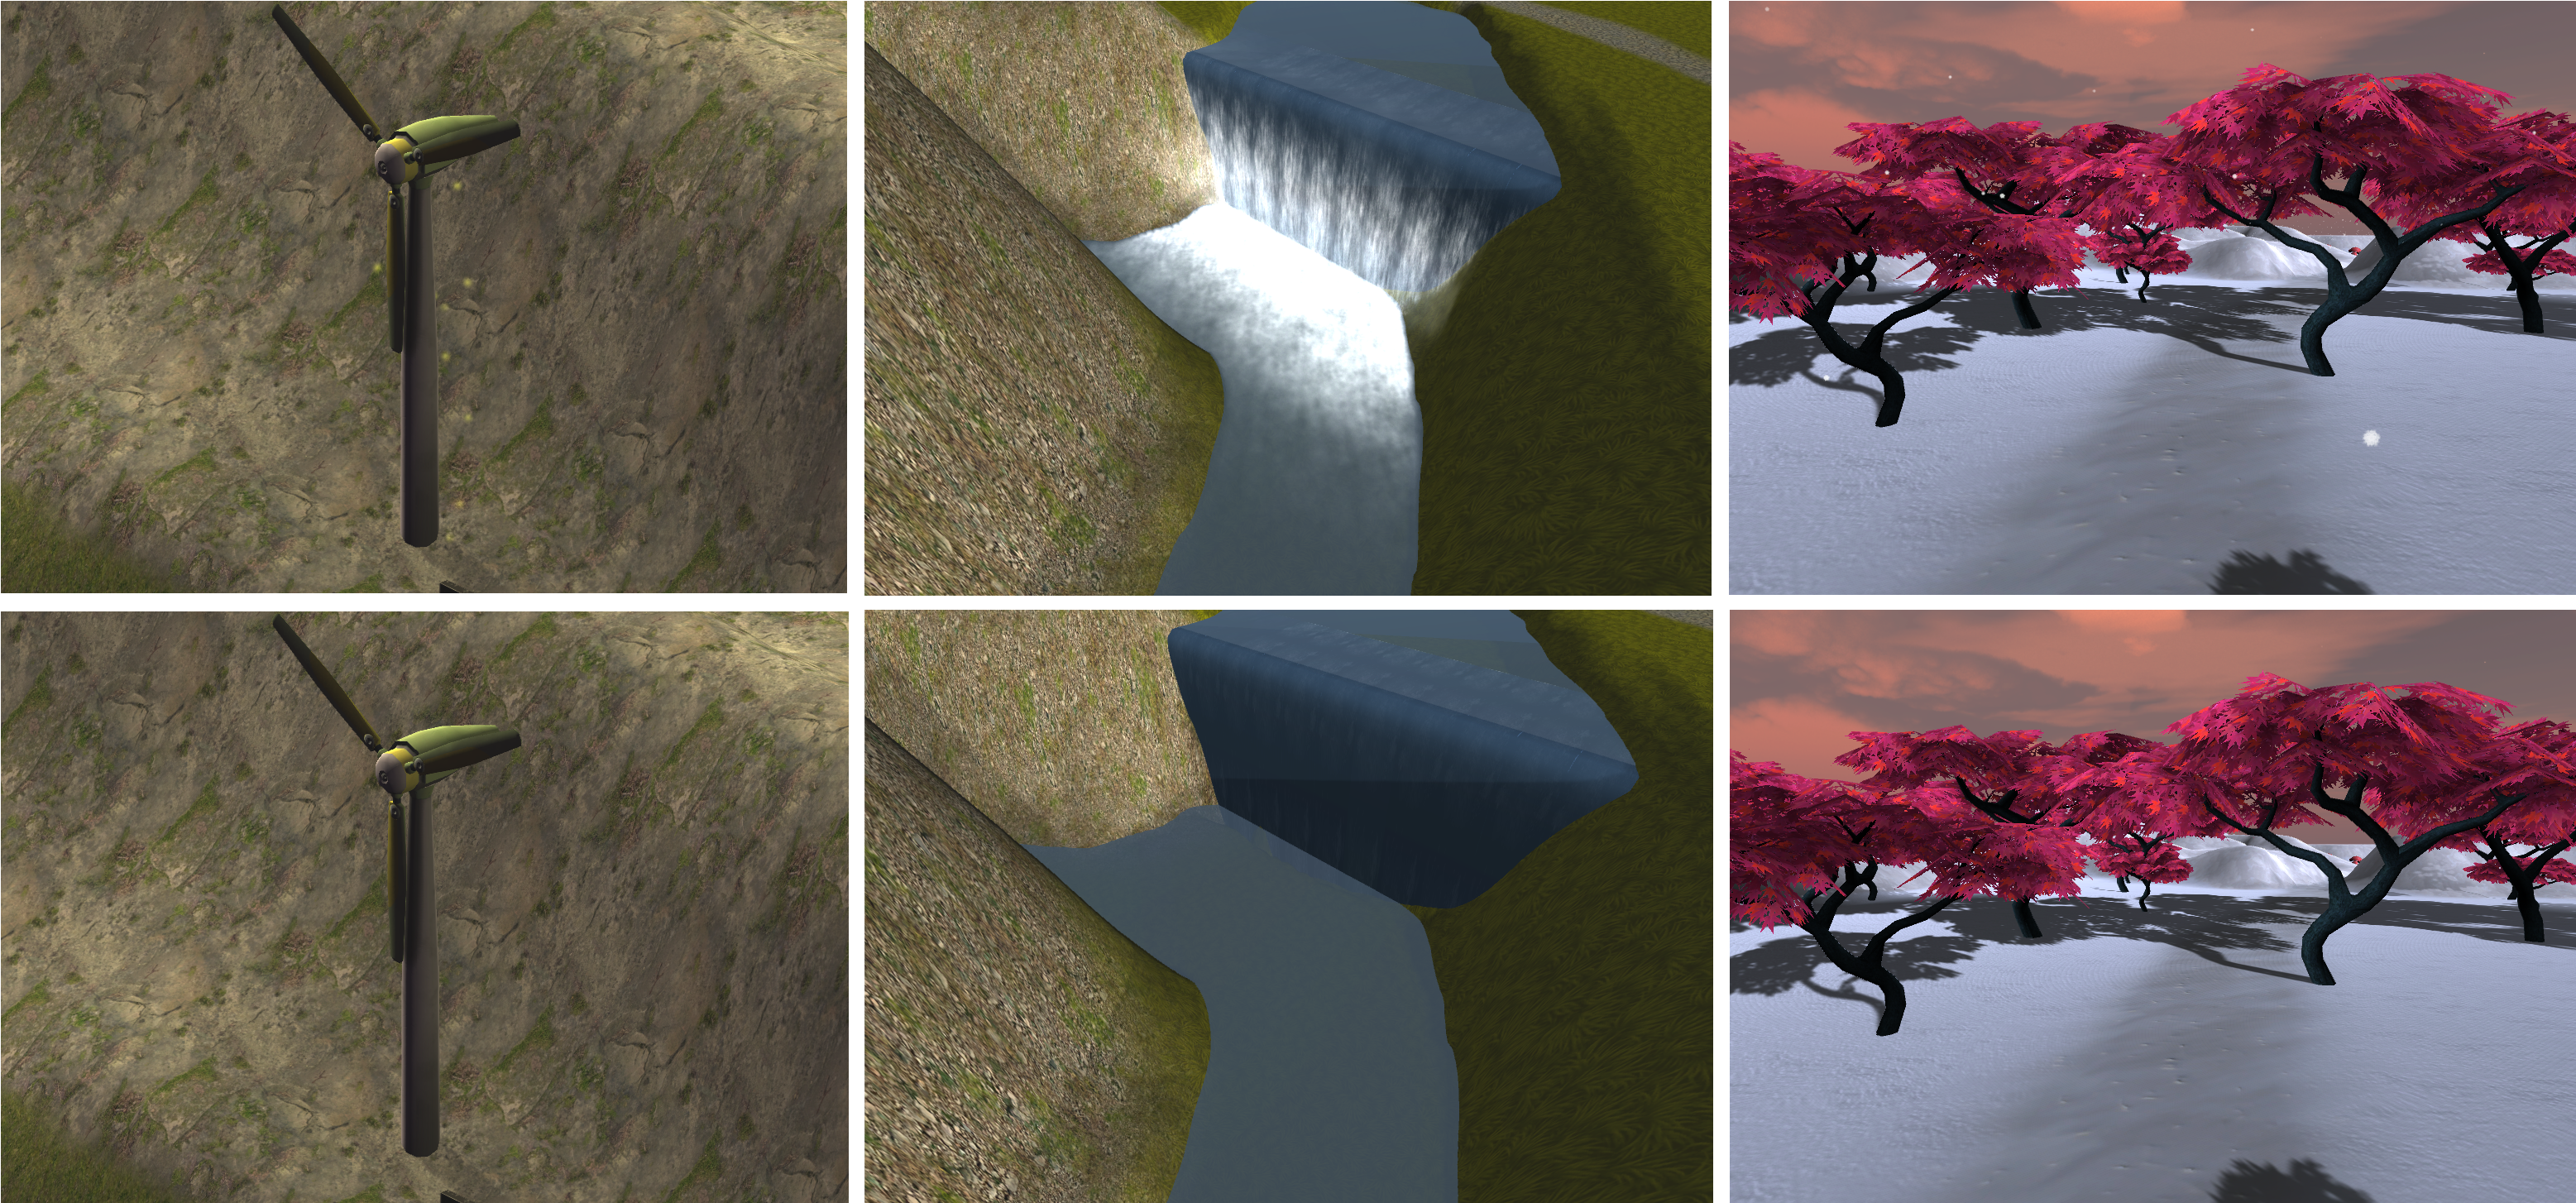
\includegraphics[height=\imgHeightMedium{}]{img/Developpement_AppauvrissementAnimation.png}}
			\captionof{figure}{Appauvrissement des particules: en haut: avec; en bas: sans.}
			\label{ParticlesImpoverishment}
		\end{minipage}\medskip	
		\\
		
		L'appauvrissement des animations active et désactive tous les animateurs de la scène qui ne possèdent pas le \textit{tag} "Guide", "Door", "Player" ou "UI". Ces différents animateurs sont essentiels au SG et gèrent, respectivement, la marche du guide, l'ouverture et la fermeture des portes, l'articulation du joueur (quand le SG est joué au clavier) et l'animation de \textit{scan} du HUD. Cela comprend les animations des objectifs telles que celle de l'éolienne. D'autres animations sont effectuées par script. C'est le cas de l'animation des poissons (monde 4 et 5), des palmiers et des vagues (monde 5). Elles n'ont donc pas de composants animateur.	
		\\
			
		Pour permettre leur activation/désactivation gérée par le script "AnimationController", il a été proposé à Monsieur K. Laipe la création d'une interface ("ScriptAnimator\_I"). Elle contient la signature d'une méthode pour l'activation et la désactivation de l'animation. "AnimationController" doit alors, en plus de tous les animateurs (\textit{Animator}), récupérer tous les éléments implémentant l'interface "ScriptAnimator\_I".
		
		Un méthode pour la récupération des tous les éléments implémentant une interface est à disposition dans la classe parente à tous scripts accrochés à un \textit{GameObject} de ce projet: "SGMonoBehaviour". Plus de détails sur cette classe sont présents dans la section \ref{sDevStructure}.	
		
		Finalement, la désactivation des animations supprime également l'effet de vent dans l'herbe.
		
	\subsection*{Paramètre d'appauvrissement général}
		Tous les appauvrissements précédemment décrits dans cette section offrent une grande possibilité de personnalisation du SG pour chaque patient. Cependant, pour l'intégration avec le LHS, il est souhaitable de n'avoir qu'un seul facteur. Ainsi le thérapeute a accès à une seule variable générale pour l'appauvrissement et n'a pas à effectuer tous ces réglages. Ceci est également plus agréable pour l'IHM si le nombre de facteur est diminué. Pour se faire, un paramètre d'appauvrissement général nommé "General impoverishment" est présent dans l'inspecteur du script "ImpoverishmentModel". Il assigne des valeurs à tous les autres paramètres. Ce paramètre va de 1 à 6. Pour chacune de ces valeurs, une sélection des valeurs de chaque paramètre d'appauvrissement est effectuée. Cette sélection est détaillée dans le tableau \ref{tableGeneralImpoverishment}.\medskip
		
		\begin{minipage}{\linewidth}
			\begin{tabular}{|l|c|c|c|c|c|c|}
				\hline
				Appauvrissement&	1&	2&	3&	4&	5&	6 \\
				général&	&	&	&	& &	\\
				\hline
				
				Géométrie des& Primitives&	\textit{Billboard}&	\textit{Billboards}&	\textit{Billboards}&	Géométrie	&	Géométrie \\
				\textit{Landscape} & 3D& &	\textit{Cloud}&	\textit{Cloud}&	complète	&	complète \\
				\textit{elements}& & & & & & \\
				\hline
				
				Géométrie&		1&	1&	2&	2&	3&	3 \\
				du terrain& & & & & & \\
				\hline
				Facteur de&		0.1&	0.3&	0.45&	0.6&	0.8&	1 \\
				quantité& & & & & & \\
				\hline
				Herbe&		\textsf{X}&	\textsf{X}&	\textsf{X}&	\textsf{X}&	\textsf{X}&	\checkmark \\
				\hline
				Animations&		\textsf{X}&	\textsf{X}&	\textsf{X}&	\textsf{X}&	\textsf{X}&	\checkmark \\
				\hline
				Particules&		\textsf{X}&	\textsf{X}&	\checkmark&	\checkmark&	\checkmark&	\checkmark \\
				\hline
				Audio&		\textsf{X}&	\textit{footsteps}&	\textit{footsteps}&	\textit{footsteps}&	Tous&	Tous \\
				&		&	& \textit{UI\_sounds}& \textit{UI\_sounds}&	&	\\
				&		&	&	&	\textit{music}&	&	\\
				\hline
				
				Lumière&		0&	1&	1&	2&	2&	2 \\
				\hline
				Nombre de &		256&	256&	256&	256&	256&	256 \\
				couleurs& & & & & & \\
				\hline
			\end{tabular}
			\captionof{table}{Réglages de l'appauvrissement d'après le paramètre général.}
			\label{tableGeneralImpoverishment}	
		\end{minipage}\medskip
		
		Ces valeurs sont choisies arbitrairement afin d'utiliser les différents aspects de l'appauvrissement. Leur sélection n'a pas été faîte suite à des tests avec le domaine médical. Elle a une valeur démonstrative et ne garantit pas d'avoir une évolution cohérente de la complexité d'interprétation de la scène pour les patients. Ce travail de sélection basé sur une réflexion en collaboration avec le domaine médicale dépasse des objectifs sélectionnés. Il pourra être réalisé dans le projet R\&D englobant.
		
		"Billb." et "Billb.C." désignent les géométrie \textit{billboard} et \textit{billboards cloud} avec normales. Les versions sans normales ne sont pas utilisées, pour que les variation d'effets de lumières ne se fassent qu'avec l'appauvrissement concerné et non la géométrie.
		
		Un aperçu des six niveaux est visible dans la figure \ref{GeneralImpoverishment}.\medskip
		
		\begin{minipage}{\linewidth}
			\makebox[\linewidth]{
				\includegraphics[width=\textwidth]{img/Poster_Appauvrissement3.png}}
			\captionof{figure}{Appauvrissement général. Dans l'ordre de lecture, de 6 à 1.}
			\label{GeneralImpoverishment}
		\end{minipage}\medskip%TODO: Refaire en vertical

\section{Éléments du SG}
	\label{sDevDeroulementPartie}
	
	Dans cette section est détaillée la façon dont sont implémentés les différents composants du SG permettant le déroulement d'un partie. Ce déroulement est également décrit dans les sous-sections concernées. L'élément principal permettant la gestion d'une partie est le script "GameController". Ce dernier est chargé en même temps qu'un niveau. Il définit notamment sa durée, grâce à son paramètre "Time Exercice Minutes". C'est lui qui gère les différents états du SG qui sont: ENTER\_ANIMATION; WAIT\_IOCONTROLLER; PLAY; PAUSE; GAME\_OVER.
	
	\subsection*{Interaction}
		Le SG contient trois interactions: le déplacement; la pause; le \textit{scan}. Pour la première, une section entière lui est consacrée (section \ref{sDevArticulation}). La deuxième existe simplement à des fins de tests, quand le LHS n'est pas disponible. La pause est normalement lancée depuis l'IHM par le thérapeute et ne concerne pas le joueur. Pour le moment, la pause peut être activée et désactivée via un appui sur la touche "P" du clavier. Aucun message ou indication n'est donné au patient, il ne peut juste plus avancer ou scanner. Son implémentation se trouve dans le script "GameController": le temps est figé et l'état passe en "PAUSE". La suite de cette sous-section détaille l'interaction du \textit{scan}.
		\\
		
		Le \textit{scan} est le moyen de valider les objectifs présents dans la scène. Un des avantages est que cela n'ajoute pas de périphérique supplémentaire, tout peut se faire avec le HMD déjà utilisé pour l'immersion. Son deuxième avantage est qu'elle correspond à une interaction naturelle qui est de regarder autour de son environnement. C'est donc probablement une des premières tâches que le patient peut accomplir en même temps que de réaliser son mouvement. Le seul élément non naturel de cette interaction est, une fois l'élément découvert, de devoir le fixer du regard jusqu'à ce que le \textit{scan} soit terminé. Cette opération dure actuellement cinq secondes mais peut être augmenté ou diminué si nécessaire.
		\\
		
		Cette interaction est implémentée à l'aide d'un lancé de rayon partant du centre de la caméra. Il est effectué dans la classe "ScannerController". Ce lancé permet de récupérer le premier \textit{collider} rencontré. Le lancé de rayon lance un \textit{scan} si le \textit{collider} rencontré est dans la couche (\textit{layer}) "Scannable". Pour qu'un élément puisse faire l'objet d'un \textit{scan}, il doit donc avoir un \textit{collider} avec la case "Is Trigger" cochée et être dans la couche "Scannable".
	
		Une fois le \textit{scan} effectué, si l'élément est un objectif, il sera alors considéré comme obtenu. Ce qui a pour conséquence la désactivation des indications d'aides (zone sur la carte et scintillement), l'indication de sa position sur la carte avec un point précis en vert ainsi que la sauvegarde persistante de l'obtention de cet objectif. Ensuite, un aperçu de cet objet s'affiche dans le HUD (voir figure \ref{GuideScan}). Cet affichage permet de visualiser l'objet dans son ensemble. En effet, pour ajouter du challenge, seuls certains éléments d'un objet peuvent être visibles. Cet affichage permet alors de réaliser ce que représente cet objet. Cette affichage dure tant que l'on regarde l'objet. Dès que l'on en détourne le regard, il disparaît progressivement. En regardant à nouveau cet objet et si aucun \textit{scan} n'a été effectué entre temps, il s'affiche progressivement sans réaliser de nouveau \textit{scan}. Cet affichage réalise, par défaut, une rotation constante de l'objet autour de l'axe y pour le voir sous plusieurs angles. Celui-ci peut être désactivé d'un objet à l'autre. Dans le SG actuel, il n'y a pas uniquement les objectifs qui peuvent être la cible du \textit{scan}. Le guide peut également l'être (figure \ref{GuideScan}). Dans ce cas, seules ses jambes sont affichées avec une vue latérale et sans rotation. Cela a pour but de permettre à l'utilisateur de se concentrer sur le mouvement et de le voir sous plusieurs angles afin d'améliorer l'activation des neurones miroirs.\medskip
		
		\begin{minipage}{\linewidth}
			\makebox[\linewidth]{
				\includegraphics[width=\textwidth]{img/Developpement_ScanGuide.png}}
			\captionof{figure}{Animation de \textit{scan} et affichage de l'objet ciblé. Dans l'ordre de lecture: ciblage de l'objet; début du scan; scan en cours; affichage des jambes; jambes en mouvement; disparition de l'affichage.}
			\label{GuideScan}
		\end{minipage}\medskip%TODO: Diminuer taille image. Mieux la décrire (surtout l'animation du scan)
		\\
		
		Chaque objet pouvant être la cible de \textit{scan} doit également posséder le script "ScannableObject". Les paramètres de ce script permettent de régler: la taille de l'objet, pour que la visualisation dans l'affiche correctement; un décalage, pour permettre de mettre l'accent sur certaines zone de l'objet; l'activation de la rotation de la caméra. Les objectifs doivent posséder le script "ObjectiveScannable" héritant de celui cité précédemment. Il permet de considérer l'objet comme un objectif et active par défaut la rotation. Cette visualisation de l'objet est réalisée à l'aide d'une caméra supplémentaire nommée "ScanDetailsCamera". Elle se trouve à la racine de la scène de sélection des niveaux. Son contenu est rendu dans une texture qui est à son tour affichée dans l'aperçu de l'objet. C'est la caméra qui tourne autour de l'objet pour effectuer la rotation. Elle ne rend que les objets étant dans la couche "Scanned". C'est le script "ScannerController" qui s'occupe de placer l'objet cible du \textit{scan} dans cette couche.
		\\
		
		Il est possible de bouger la caméra à l'aide de la souris. Ceci permet le développement du SG sans avoir une disponibilité constante du HMD. Pour cela, il suffit de d'activer le \textit{GameObjet} "WithoutOculus" se trouvant dans celui nommé "IO" à la racine de la scène de sélection des niveaux. Attention à bien le désactiver quand le HMD est utilisé.
		\\
		
		Un dernier aspect est lié à la réalisation de cette interaction: l'animation de l'avatar. Pour améliorer l'immersion et renforcer la cohérence, il est souhaitable que l'avatar s'articule de façon à regarder dans la même direction que la caméra.
		De plus, il est souhaitable que le patient puisse, en regardant vers le bas, voir ses jambes (celles de l'avatar). Cela implique d'appliquer des rotations aux différentes articulations de l'avatar, en partant du bas du dos jusqu'au cou. Ceci a été réalisé dans le script "BodyLookOrientationController" attaché au joueur. Ce dernier nécessite une référence pour l'articulation du cou ainsi qu'un tableau de références pour la colonne vertébrale (figure \ref{AvatarArticulationLook}). Cela a pour but d'être compatible avec plusieurs avatars articulés de différentes façons. La rotation nécessaire est alors divisée sur ces différentes articulations de la façon suivante: chaque partie "i" de la colonne vertébrale a un poids de "i" et le cou a un poids de 2*n; où "n" est le nombre de segments de la colonne et "i" allant de 1 (bas du dos) à "n" (haut du dos). %TODO: Mettre en forme cette "équation"
		Ceci amène à une rotation principalement effectuée au niveau du cou mais tout de même accompagnée par la colonne vertébrale. Cette répartition a été faite de façon expérimentale avec le modèle ayant quatre segments pour la colonne vertébrale. Une fois la rotation appliquée, si celle-ci ne tourne pas uniquement autour de l'axe "y", l'emplacement des yeux ne correspond plus à celui de la caméra. Celle-ci est donc déplacée de façon à correspondre. Si l'articulation de l'avatar ne se fait pas de façon naturelle, ce déplacement pourrait induire un malaise suite à des mouvements rapides et répétés.
		\medskip
		
		\begin{minipage}{\linewidth}
			\makebox[\linewidth]{
				\includegraphics[height=\imgHeightMedium{}]{img/Developpement_ArticulationRegard_Contrast.png}}
			\captionof{figure}{Articulation de l'avatar d'après le regard.}
			\label{AvatarArticulationLook}
		\end{minipage}\medskip	
		
		
		Pour améliorer cette position, l'utilisation du traqueur de position fournit avec l'\textit{Oculus Rift} a été envisagée. Celui-ci induisait cependant une difficulté supplémentaire par rapport à l'articulation. On devait alors faire correspondre non seulement l'orientation mais également la position. Pour cela, il faudrait résoudre des problèmes de cinématique inverse de complexité grandement supérieure \cite{wikipedia_cinematiqueInverse, Buss_InverseKinematicIntro}. D'autre problèmes se posent également avec l'utilisation de ce traqueur, notamment son installation avec le LHS ou encore son comportement hors limite du capteurs (de brusques sauts sont présents par défaut). Pour ces différentes raisons, il a été décidé de ne pas l'utiliser et de se contenter du déplacement induit par les articulations du dos et du cou.
		
	\subsection*{Zone familière}
		La zone familière a été réalisée à l'intérieur du vaisseau spatial. Ce dernier est choisi car il possède une longue zone plate au niveau du terrain. Cet aspect est idéal pour y placer des salles permettant de rejoindre la sortie du vaisseau sans pente ni escalier. Pour l'ouverture du vaisseau, elle se fait à l'aide d'une rotation de la dernière porte, visible dans la figure \ref{Spaceship}. Le modèle 3D du vaisseau a été grossièrement coupé pour permettre une cohérence avec la porte.
		\medskip
		
		\begin{minipage}{\linewidth}
			\makebox[\linewidth]{
				\includegraphics[height=\imgHeightSmall{}]{img/Developpement_Spaceship_Contrast.png}}
			\captionof{figure}{Vaisseau spatial et ouverture de la porte frontale.}
			\label{Spaceship}
		\end{minipage}\medskip
		
		Les murs et les portes des pièces intérieures sont entièrement réalisés à l'aide de primitives 3D disponibles dans \textit{Unity}. La création de ces pièces sur un logiciel de modélisation 3D serait souhaitable mais requiert les compétences d'un \textit{designer}. Cette zone (visible dans la figure \ref{Interior}) est constituée de trois pièces: sélection du niveau; chambre; sas. Elle contient également trois portes menant d'une zone à la suivante. L'éclairage consiste en une lumière ponctuelle par pièce. Cette lumière n'éclaire pas les objets dans la couche "Terrain" ni ceux dans celle "Default". La première pièce est celle de départ et de fin de niveau. Elle contient un écran utilisé pour la sélection du niveau (contre la porte) et un autre écran pour l'affichage du score (contre le mur). La deuxième pièce contient différents éléments familiers faisant le lien entre l'environnement hospitalier et l'environnement étranger des planètes inconnues. Les objets familiers sont les suivants: une armoire; un bureau; une fausse plante; un tableau; une photo de famille. La dernière pièce est un couloir vide donnant accès, une fois la porte ouverte, sur le monde choisit.\medskip
		
		\begin{minipage}{\linewidth}
			\makebox[\linewidth]{
				\includegraphics[height=\imgHeightMedium{}]{img/Developpment_Interior_Detoured.png}}
			\captionof{figure}{Zone intérieure, composée des trois pièces. De droite à gauche: sélection des niveaux; chambre; sas.}
			\label{Interior}
		\end{minipage}\medskip
		\\
		
		Durant une partie, le joueur doit d'abord choisir un niveau (interaction et transition détaillée dans la section \ref{sDevStructure}). Une fois la scène chargée, le SG est dans l'état "ENTER\_ANIMATION". Puis, le vaisseau atterrit puis il passe dans l'état "PLAY", excepté si le LHS n'est pas prêt, où il passe dans l'état "WAIT\_IOCONTROLLER" en attendant. Une fois dans l'état "PLAY", la porte s'ouvre, le joueur peut avancer, rejoindre le guide dans la pièce suivante et réaliser tout le parcours.		
		
	\subsection*{Parcours}
		Pour être guidé sur le parcours, le joueur et le guide contiennent chacun un objet "PathBrowser". Ces objets leur donnent leur déplacements effectué depuis le dernier appel. Ces déplacements sont donnés par une position et une orientation. Celles-ci sont définies dans l'objet "Path" composé d'un tableau de "PathSegment". Durant une partie, c'est une instance de "PathLevel" qui est créée. Celle-ci définit trois segments. Le premier permet d'aller du point "LevelSelectionPoint" à "MainGatePoint" (dans le vaisseau spatial). Le deuxième segment est celui du terrain. Et le troisième est l'inverse du premier, permettant d'aller de l'entrée du vaisseau au tableau des scores. Cette structure de classe est détaillée dans la figure \ref{PathClassDiagram}.\medskip
		
		\begin{minipage}{\linewidth}
			\makebox[\linewidth]{
				\includegraphics[height=\imgHeightMedium{}]{img/Developpement_PathClassDiagram_Resized.png}}
			\captionof{figure}{Diagramme de classes UML des classes utilisées pour la gestion du chemin}
			\label{PathClassDiagram}
		\end{minipage}\medskip%TODO: Mettre en annexe
		
		En début de partie, le vaisseau atterrit de manière à s'aligner avec le début du parcours. La transition entre le premier et le deuxième segment est donc assurément fluide. Pour que la transition entre le deuxième et le troisième soit également fluide, il faut s'assurer que le tracé du terrain donne la même orientation initiale que finale (bien que tournée de 180°). Ce tracé est fait dans un fichier ".svg" (étant un fichier de type XML) à l'aide du logiciel de dessin vectoriel "\textit{Inkscape}" \cite{Inkscape_website}. 		
		Une fois le tracé dessiné (contraintes expliquées plus bas dans cette sous-section), deux étapes sont à effectuer. Le dessin est exporté en bitmap au nom de "PathmapWorldX.png" et le fichier de dessin (.svg) est renommé en "path\_WorldX.xml" (pour pouvoir être importé par \textit{Unity} comme \textit{text asset}). Ces deux fichiers sont placés dans le répertoire "Terrain" et référencés dans l'objet préfabriqué "LevelX". Le fichier bitmap est affiché sur la carte quand le niveau est chargé. Le fichier XML subit plus de traitements, pour finalement projeter le tracé sur le relief du terrain. Ces traitements consistes à extraire les différents points de la courbes et leur points de contrôle et de discrétiser ces courbes d'après l'équation des courbes de Bézier cubiques \cite{CompAlg} (équation utilisée pour leur dessin). Chaque segment est alors discrétisé en 100 points et 100 directions. La raison de cette discrétisation est que l'équation donnant la position d'après le chemin parcouru (nécessaire au SG) est de complexité bien supérieure. Ce traitement est effectué dans la classe "SVGTools". La projection, bien que visible sur tous les mondes, est mieux illustrée sur le monde 1 car c'est le seul monde avec des pentes sur le chemin. Cette visualisation du chemin (figure \ref{PathInGizmos}), est visible uniquement dans l'éditeur de scène "\textit{Gizmos}", grâce au script "DrawPath". Les points et directions sont stockés dans l'instance de "PathSegmentTerrain". L'interpolation entre ces points et directions est linéaire et est réalisée par l'instance de "Path".\medskip
		
		\begin{minipage}{\linewidth}
			\makebox[\linewidth]{
				\includegraphics[height=\imgHeightSmall{}]{img/Developpement_CheminTrace.png}}
			\captionof{figure}{Tracé du chemin, tel qu'il est perçu dans \textit{Gizmos}.}
			\label{PathInGizmos}
		\end{minipage}\medskip
		
		Le dessin du chemin peut être réalisé avant ou après la création du terrain. Dans les deux cas, des contraintes doivent être respectées. Premièrement, le chemin doit être effectué en une seule courbe de Bézier. Deuxièmement, le chemin doit boucler en un point (le point final étant au même emplacement que le point de départ). Le point de contrôle du point initial et du le point final doivent être sur une même droite, du même côté du point (initial et final). Troisièmement, chaque autre point de la courbe doit avoir deux points de contrôles. Le point et ses points de contrôle doivent être sur une même droite, ces deux derniers étant chacun d'un autre côté du point (option "rendre doux les nœuds sélectionnés"). Ceci se vérifie visuellement sur la figure \ref{PathDrawing}. On y voit chaque point (autre que l'initial et le final) représenté par un carré. Finalement, le fichier de dessin doit être de 512 sur 512 (pixels). Cette page représente le terrain, il est donc souhaitable que la courbe tracé ne s'approche pas des bords. Le point initial doit également veiller à laisser suffisamment de place derrière lui pour que le vaisseau spatial soit bien intégré au terrain. Sans être une contrainte fonctionnelle, il est préférable d'avoir un chemin assez lisse et d'éviter les virages trop serrés. Ainsi le changement d'orientation automatique est plus doux pour le joueur et diminue le risque de nausées.%TODO: Retrouver une ref.
		\medskip
		
		\begin{minipage}{\linewidth}
			\makebox[\linewidth]{
				\includegraphics[height=\imgHeightSmall{}]{img/Developpement_DessinChemin.png}}
			\captionof{figure}{Aperçu du tracé sous \textit{Inkscape}. Dans l'ordre de lecture: sur fond blanc; sur une capture d'écran; sur la \textit{splatmap}.}
			\label{PathDrawing}
		\end{minipage}\medskip
		
		Si ce tracé est dessiné avant que le terrain soit créé, on peut alors modéliser le terrain autour de ce chemin dans l'éditeur. Il faut faire attention à minimiser les pentes ou à les rendre lisses, même si elles n'ont aucune influence sur l'exercice pour le moment. Si ce tracé est réalisé après le terrain, il peut être dessiné sur une capture d'écran du terrain ou sa \textit{splatmap}. Cette dernière peut être récupérée en sélectionnant le \textit{GameObject} possédant le terrain, puis en effectuant l'action "NWTools, Terrain, Export Splatmap". Elle est créée dans le dossier "Assets" au nom "splatmap.png". Les trois possibilités sont montrées dans la figure \ref{PathDrawing}.
		\\
		
		Comme le montre le diagramme de classe (figure \ref{PathClassDiagram}), chaque segment définit un objet sol (script "Ground") qui est responsable du son à lancer lors d'un pas sur ce segment. Il a également été expliqué que les hauteurs ne pouvaient pas être données et que celles du terrain étaient utilisées. Or, une autre possibilité existe pour modifier un ou deux de ces aspects. Celle-ci est utilisée pour le pont du monde 2. On remarque qu'on ne suit pas la hauteur du terrain et que les bruits de pas ne sont plus les mêmes. Ceci est possible grâce aux "PathModifier". Tout objet placé sur le chemin et modifiant la hauteur ou le son possède ce script. Il doit aussi contenir un \textit{collider} définissant sa zone. Ce dernier doit être dans la couche "HeightModifiers".
		Une fois le chemin discrétisé et projeté, une étape supplémentaire est réalisée. Pour chaque point, un lancé de rayon est effectué. Le rayon est lancé depuis les coordonné x et z du point ainsi que la hauteur maximum possible du terrain en y. Il est lancé en direction du point. S'il touche un \textit{collider} dans la couche "HeightModifiers" avant de toucher le sol, ce point prend pour hauteur celle du script "PathModifier" attaché à son \textit{GameObjet} ainsi que son objet "Ground".
		
		%TODO: Parler avec plus de détails du calcul des splines
	
	\subsection*{Placement des éléments du jeu}
		Différents éléments du SG se placent dynamiquement d'après un potentiel profil du patient. Celui-ci est à définir dans "PatientProfileModel". On peut y choisir de quel côté placer la carte, l'aperçu des objectifs et la répartition gauche/droite des objectifs. Le choix du côté est directement lié à l'héminégligence du patient et peut évoluer au fil de la réhabilitation. Au début, les informations importantes doivent être mises du côté non négligé. Puis, avec le temps, on peut en déplacer du côté négligé pour demander au patient d'aller y chercher des informations.
		Bien que ces trois possibilités existent dans le SG, seule la répartition des objets fut définie comme pertinente pour un paramètre de l'IHM. Ceci du moins pour une première version. Comme il sera expliqué dans le chapitre "Résultats", l'intégration avec le LHS n'a pas pu être effectuée. Ce paramètre n'est donc pas non plus récupéré pour le moment. Il ne peut donc pas être modifié uniquement depuis l'inspecteur, dans \textit{Unity}.
		\\
	
		Pour l'affichage de la carte et l'aperçu de l'objectif, une sélection "gauche ou droite" est effectuée. Pour le placement des objectifs, le paramètre est un nombre réel allant de -1 à 1. Ce paramètre est "Balance Objectives" de l'inspecteur du script "PatientProfileModel" présent dans le \textit{GameObject} "Models" dès la scène de chargement des niveaux. Si ce paramètre est à -1, tous les objectifs seront à gauche. S'il est à 1, ils seront tous à droite. La progression est linéaire, on obtient alors un équilibre entre gauche et droite quand il vaut 0. Bien que cette distribution gauche/droite est respectée, les objets allant d'un côté ou de l'autre sont choisis aléatoirement. D'une exécution à l'autre, il est possible que des objets changent de côté. C'est le "GameController" qui, au chargement du niveau, place les objectifs. Chaque objectif possède le script "ObjectiveScannable" proposant une position, une orientation et une source audio pour chaque côté du chemin. Ces valeur sont à entrer manuellement. Une fois le niveau chargé, l'objectif sera déplacé et orienté en fonction et la bonne source audio sera activée. Ces sources audio ont été configurées par Monsieur Laipe. La position des objectifs dans la scène n'a pas d'influence, seules ces valeurs sont utilisées. On peut voir un aperçu du placement et des sources audio sur la figure \ref{ObjectivesPlacement}. Le premier objectif rencontré, se situe sur les terres sortant de l'eau s'il est à gauche. S'il est à droite, il est alors plus proche, sur le flan de la montagne nous séparant du lac. On remarque que l'objectif étant plus proche à droite, il possède une source audio avec une plus faible portée. \medskip
		
		\begin{minipage}{\linewidth}
			\makebox[\linewidth]{
				\includegraphics[height=\imgHeightSmall{}]{img/Developpement_ObjectivePlacement.png}}
			\captionof{figure}{Placement des objectifs et leur source audio sur le monde 4, parcours allant dans le sens des aiguilles d'une montre. À gauche, objectifs à gauche du chemin; à droite, objectifs à droite du chemin}
			\label{ObjectivesPlacement}
		\end{minipage}\medskip
		
	
	\subsection*{Placement des \textit{landscape elements}}
		Le référencement des \textit{landscape elements} se fait par famille (script "LandscapeElementFamily"). Trois familles peuvent être utilisées par niveaux. Leurs zones et concentration peuvent être définies. Ces familles sont composées de \textit{landscape elements} (script "LandscapeElement"). Les éléments placés dans la zone de la famille, y sont choisi aléatoirement. Les familles utilisées dans ce projet ne contiennent souvent qu'un élément. Les champignons du monde 3 sont un exemple de famille en contenant plusieurs.
		\\
	
		Le placement des \textit{landscape elements} se fait à l'aide d'une texture indiquant les différentes zones les contenant, appelée "LandscapeElementsMaps". Trois familles peuvent être utilisées par niveau (correspondant aux trois canaux rouge, vert, bleu). Le choix d'utiliser une texture est lié à la possibilité future de génération des mondes. En effet, pour générer les mondes, une des possibilités déjà explorée (voir section \ref{sDevAppauvrissement}) est de générer deux textures. Celles-ci étant une \textit{heightmap} et une \textit{splatmap} décrivant respectivement les hauteurs et les textures.
		Cette texture est réalisée en partant d'une capture d'écran du terrain ou de sa \textit{splatmap} (si l'on souhaite faire correspondre une texture de sol avec une famille). Celle utilisée pour le monde 1 est visible dans la figure \ref{LandscapeElementsMap}. Aucun objet ne sera placé dans les zones en noir. On voit distinctement le chemin du niveau avec une grande épaisseur en noir, ainsi aucun objet ne sera placé sur le chemin. Même raisonnement pour le vaisseau spatial se plaçant en début de chemin. Les zones de dégradés entre les couleurs permettent de mélanger plusieurs familles. Les zones de dégradés sur le noir permettent de diminuer la concentration d'objet dans cette zone.\medskip
		
		\begin{minipage}{\linewidth}
			\makebox[\linewidth]{
				\includegraphics[height=\imgHeightSmall{}]{img/Developpement_LandscapeElementsMap.png}}
			\captionof{figure}{Textures du placement des \textit{landscape elements} ("\textit{LandscapeElementsMap}")}
			\label{LandscapeElementsMap}
		\end{minipage}\medskip
		
		Pour générer les objets, il faut être dans la scène, sélectionner l'image et exécuter l'action "NWTools/Terrain/Apply GameObjectMap" implémentée dans le script "ApplyGameObjectMap". Cette action tire premièrement un point aléatoire pour 16 pixels. Les images créées étant de 512 pixels par 512, cela fait 16'384 pixels. À chacun de ces pixels est ensuite attribué une couleur rouge, vert ou bleu. Ceux étant dans le noir sont ignorés. Pour ceux possédant des dégradés, la couleur est tirée aléatoirement avec une distribution correspondant au dégradé. Ensuite, la liste est parcourue. Pour chaque élément non vide, deux actions sont effectuées. Premièrement, un \textit{landscape element} correspondant (tiré aléatoirement dans la famille) est attribué. Deuxièmement, tous les points de la liste étant à moins de "minRadiusNeeded" sont mis à \textit{null}. Cette variable est définie pour chaque \textit{landscape element} et définit à quelle distance minimum peut être instancié un autre \textit{landscape elements}. Les \textit{landscape elements} générés sont des instances des objets préfabriqués "Referencer". Ils sont instanciés dans la hiérarchie de \textit{GameObjects}: "World/Terrain/Landscape elements" et sont triés par famille. Pour visualiser les éléments générés, il faut lancer la scène, soit depuis la sélection des niveaux, soit en y intégrant temporairement les objets préfabriqués "Models" et "ImpoverishmentControllers".
		
		La quantité d'éléments placés correspond à la quantité "2" du facteur d'appauvrissement quantitatif, soit deux fois la quantité normale du SG (voir section \ref{sDevAppauvrissement}). Si l'on remarque que la scène est trop chargée (même avec le facteur mis à "1"), il faut alors recommencer l'opération avec des valeurs "minRadiusNeeded" plus grandes pour les \textit{landscape elements} utilisés. Avant de relancer la génération, il faut supprimer le \textit{GameObject} "World/Terrain/Landscape elements".
		\\
		
		L'action de génération se nomme "ApplyGameObjectMap" car une première version a été implémentée précédemment. Celle-ci se nommait "ApplyTreeMap" et plaçait non pas des \textit{GameObjects} dans la scène mais des objets "Tree" utilisés par le terrain \textit{Unity}. Le principal désavantage de cette méthode était la création automatique de niveaux de détails qui posait des problèmes d'incohérence avec les appauvrissement (\textit{e.g.}, à partir d'une certaine distance, les arbres étaient remplacés par des \textit{billboards}).	
	
	\subsection*{Fin de partie et calcul de score}
		Chaque partie se termine devant l'écran des scores, le HUD est désactivé et l'écran affiche notre score. Cet écran se trouve à l'opposé de l'écran de choix des niveaux (dans la même pièce). Le SG reste ainsi jusqu'à ce qu'il soit fermé. Ce qui pourra se faire, une fois l'intégration au LHS faîte, quand l'exercice "SG" est considéré terminé et que le robot entre dans l'état d'attente d'exercice. Un niveau correspondant à une session de jeu, soit un exercice (du point de vue IHM), le SG devra être fermé entre chaque.%TODO: Changer ça si intégration faîte
		\\
		
		L'écran affiche donc le détail de notre score. Quatre éléments sont calculés pour le score final. Deux en relation des objectifs et deux en relation avec la marche. Le plus important et servant de base pour l'unité utilisée dans ce calcul est liée à la marche et représente le temps restant. Un point est attribué par seconde restante. Si le temps est écoulé ou que l'exercice est interrompu par un thérapeute (détails des cas de figure, plus bas dans cette sous-section) un malus est attribué. Ce malus correspond au nombre de secondes nécessaires pour finir le niveau d'après la vitesse moyenne. Ce malus ne peut pas excéder le temps maximum du niveau.
		
		Le deuxième score calculé est un bonus et peut aller de 0 à 180. Il est calculé par le temps passé à effectuer un mouvement sur le temps total. Ainsi, si un patient n'arrive pas à terminer le niveau mais n'a marqué aucune pause, il reçoit l'équivalent de trois minutes restantes. Le patient pouvant effectuer des mouvements saccadés, les arrêts de moins de deux secondes ne sont pas considérés comme des moments de pause. Ce temps est définit dans le paramètre "Time To Idle" du script "PlayerController".
	
		Les deux points restants concernent les objectifs. Ce sont deux facteurs compris entre 0 et 1. Ils forment à eux deux un seul bonus se multipliant mutuellement, puis à 180. Le premier facteur est le nombre d'objectifs obtenus sur le nombre total du niveau. Le deuxième est le nombre de \textit{scan} effectués sur le nombre total de ceux tentés. Ainsi, si le joueur arrive à effectuer un \textit{scan} de tous les objectifs du premier coup, il reçoit également l'équivalent de trois minutes restantes.
		
		L'affichage de ces bonus est visible dans la figure \ref{ScoreScreen}. Pour avoir un tel score, il faut avoir: terminé son niveau avec une minute d'avance; passé les deux tiers de son temps à effectuer un mouvement de marche; obtenu les trois quarts des objets; effectué un \textit{scan} échoué (en moyenne) par objectif finalement obtenus.\medskip
		
		\begin{minipage}{\linewidth}
			\makebox[\linewidth]{
				\includegraphics[height=\imgHeightSmall{}]{img/Developpement_Score.png}}
			\captionof{figure}{Écran d'affichage des scores, en fin de partie.}
			\label{ScoreScreen}
		\end{minipage}\medskip
		\\%TODO: Plus grand peu être ?
		
		Une partie peut se terminer de trois façons différentes. La première, la plus simple est la réalisation complète du parcours. Dès que le joueur atteint son point de départ à l'intérieur du vaisseau, la partie est terminée (il ne peut plus avancer, le HUD se masque et les scores s'affichent). La deuxième se produit lorsque le temps est écoulé, ce dernier étant affiché sous forme de barre d'oxygène dans le HUD. La dernière façon est l'interruption par le thérapeute de l'exercice. Dans les deux derniers cas, le joueur n'est pas dans le vaisseau spatial, devant l'affichage des scores. Il doit y être non seulement pour les visualiser mais également pour apporter une transition entre un environnement étranger (planète inconnue) et la salle réelle.
	
		Pour placer le joueur à l'endroit souhaité, il est déplacé rapidement avec un effet de téléportation. Ce déplacement est géré par le script "TeleportationController", en trois phases. La première initie la téléportation en faisant apparaître des "anneaux de téléportation". Ceci est effectué en deux secondes avec un fondu influant sur sa transparence. Puis le déplacement restant (en suivant le chemin) est effectué en trois secondes avec un effet de flou de mouvement. Finalement, les anneaux disparaissent en deux secondes également.
		
		Pour le flou de mouvement, il est réalisé à l'aide du script "MotionBlur" attaché à la caméra. Ce script provient du paquet "ImageEffects" proposé dans les "Standard Assets" de \textit{Unity}.
		
		Les anneaux sont deux tores animés. Ils sont réalisés à l'aide de peu de polygones sous \textit{Blender} \cite{Blender_website}, ce qui leurs donne un effet de pentagone plutôt que de cercles. Leur animation consiste en une rotation autour de l'axe "y" ainsi qu'un déplacement de haut en bas. L'un est placé à une hauteur légèrement plus grande que la taille du joueur et va vers le bas tandis que l'autre commence à zéro et monte. Ces anneaux sont instanciés dans la scène en tant qu'enfant du joueur ce qui leur permet de le suivre dans les déplacements provoqués par la téléportation. Leur \textit{material} utilise le \textit{shader} "Standard" avec une couleur bleue claire et émet une lumière de la même couleur. Concrètement ils se placent autour du joueur, visible dans la figure \ref{Teleportation}.\medskip
	
		\begin{minipage}{\linewidth}
			\makebox[\linewidth]{
				\includegraphics[height=\imgHeightMedium{}]{img/Developpement_Teleportation.png}}
			\captionof{figure}{Visualisation des anneaux de téléportation et de ses différentes étapes. Dans l'ordre de lecture: anneaux à deux moments de leur animations; barre d'oxygène vide; disparition du HUD et apparition des anneaux; flou de mouvement.}
			\label{Teleportation}
		\end{minipage}\medskip%TODO: Spéarer en plusieurs images ?
	
	\subsection*{Visualisation de la progression}
		La progression du joueur dans le SG peut d'abord se voir dans l'écran de sélection du niveau. Pour chaque niveau, le joueur voit les objectifs qu'il a déjà obtenus et un contour de ceux à obtenir. Ces aperçus sont stockés sous forme d'objets préfabriqués dans "Prefabs/UI/ObjectiveViews". Ils sont référencés dans chaque objet préfabriqué "LevelX". L'image de l'objectif est générée à l'aide de la scène "ObjectiveViewGenerator" de la même façon que le sont les \textit{billboard cloud} (voir section \ref{sDevAppauvrissement}). Elle est générée dans le dossier "Assets/Textures/UI/Objectives/Gen/". Les contours sont dessinés à l'aide d'un logiciel (en l'occurrence \textit{Inkscape} \cite{Inkscape_website}) externe avec, pour base, l'image de l'objectif. La figure \ref{ProgressionAtLevelSelection} montre un aperçu de l'écran de choix des niveaux indiquant cette progression.\medskip
		
		\begin{minipage}{\linewidth}
			\makebox[\linewidth]{
				\includegraphics[height=\imgHeightSmall{}]{img/Developpement_ProgressionChoixNiveau.png}}
			\captionof{figure}{Écran de choix du niveau, visualisation des objectifs déjà obtenus et ceux restant à obtenir.}
			\label{ProgressionAtLevelSelection}
		\end{minipage}\medskip
		\\
		
		Durant une partie, L'emplacement de ces objectifs est indiqué sur la carte du HUD (figure \ref{ProgressionInGame}).
		S'ils ne sont pas encore obtenus, une zone dans laquelle ils peuvent se trouver est présentée (les trois zones grises sur la première image de la figure \ref{ProgressionInGame}). S'ils ont déjà été obtenus, un point vert montre leur emplacement (les deux premiers objets sur l'image de droite de la figure \ref{ProgressionInGame}). Certains objectifs affichent des indications uniquement après qu'un certain nombre d'objectifs de ce niveau aient été obtenus. Ils possèdent le script "UnlockableObjectiveScannable" héritant de "ObjectiveScannable". Ce script définit le nombre d'objectifs nécessaires avant l'apparition des indications à l'aide du paramètre "Nb To Scan Before Showing". C'est le cas du dernier objectif du monde 1, que l'on voit apparaître après le \textit{scan} des deux premiers. Cette apparition est également visible dans la figure \ref{ProgressionInGame}.\medskip
		
		\begin{minipage}{\linewidth}
			\makebox[\linewidth]{
				\includegraphics[height=\imgHeightMedium{}]{img/Development_InGameProgression.png}}
			\captionof{figure}{Carte de visualisation de la progression durant une partie.}
			\label{ProgressionInGame}
		\end{minipage}\medskip%TODO: Refaire avec la flèche droite ? Et un fond moins sombre ?
		
		Le dernier moyen de visualiser sa progression durant une partie est avec l'aide de la flèche présente sur la carte (également visible dans la figure \ref{ProgressionInGame}). Elle affiche notre emplacement sur le chemin. Il est ainsi possible de se situer dans le déroulement de la session de jeu.
		
		%TODO: Parler de la jauge d'oxygène également ? pour dire qu'on peut ainsi évaluer son on doit se dépecher ou pas pour finir le niveau.

\section{Articulation de l'avatar et animation de marche}
	\label{sDevArticulation}
	Cette section décrit l'implémentation du mouvement de marche. Le mouvement du guide et celui du joueur étant différents, ils sont chacun décrit dans une sous-section appropriée. Celui du joueur est censé correspondre au mouvement du LHS. Cependant, pour le test un déplacement au clavier est implémenté. Le mouvement lié à ce déplacement possède également sa propre sous-section. Finalement, le calcul du déplacement du joueur d'après ce mouvement est décrit.
	\subsection*{Articulation du guide}
		Les mouvements du guide sont issus d'une animation provenant du paquet "Raw Mocap Data". Ce dernier est mis à disposition par \textit{Unity} sur l'\textit{asset store} \cite{RawMocapData_assetStorePage} et se trouve dans le dossier "Plugins" de ce projet. Il contient diverses animations pouvant être utilisées pour des avatars humanoïdes. De base, ces dernières contenaient un déplacement du modèle ce qui ajoutait un déplacement supplémentaire à celui géré par "GuideController" pour suivre le chemin. L'animation contenait plusieurs pas et les derniers étaient effectués en reculant. L'animation a donc été coupée pour avoir uniquement deux pas pouvant être mis en boucle tout en tentant de ne pas voir de coupure. Le déplacement a également été supprimé. La vitesse de déplacement du modèle fut ensuite adaptée pour correspondre au rythme de marche. Actuellement l'animation est effectuée sans synchronisation avec les jambes de l'avatar.
		\\
		
		Le guide possède également une animation "Idle" lancée quand il attend le joueur. Le guide possède une distance maximale à laquelle il doit attendre le joueur et une minimale à laquelle il doit repartir. Il est théoriquement possible, si le joueur se déplace très rapidement de dépasser le guide. Ceci est dut au fait que sa vitesse de marche est constante. Ce cas est cependant peu probable, les patients auront une vitesse probablement bien inférieure \cite{Eng_GaitTrainingStrategies_WalkingSpeed}. L'adaptation du guide à une vitesse relative à celle du patient sera dans tous les cas un point important, une fois le SG interfacé avec le LHS.
		
	\subsection*{Articulation du joueur avec le LHS}
	
		L'articulation du joueur se fait à l'aide des différents angles récupérés du LHS. La mesure de ces angles est visible sur la figure \ref{LHSAngles}. On remarque que le sens trigonométrique strict n'est pas toujours respecté. Le patient est assis sur un siège, dont l'assise empêche l'angle T1 d'aller en dessous de Td (angle fixe). Le mouvement, pour être corrigé, doit donc soustraire Td à T1. Cet angle fixe est récupéré une seule fois comme donnée statique du patient et correspond à la variable "\textit{backAngle}".\medskip
		
		\begin{minipage}{\linewidth}
			\makebox[\linewidth]{
				\includegraphics[height=\imgHeightBig{}]{img/LHS_angles3_Resized.jpg}}
			\captionof{figure}{Schéma de la mesure des différents angles des articulations du patient, d'après le LHS.}
			\label{LHSAngles}
		\end{minipage}\medskip
		
		Ce sont ces angles qui sont récupérés par le programme lisant l'application temps réel du LHS. Ils sont placés dans un objet "PatientState" où les angles T1, T2, T3 correspondent respectivement aux articulations "\textit{Hip}", "\textit{Knee}" et "\textit{Ankle}" (hanche, genou et cheville).
		
		L'articulation de l'avatar, est un peu plus compliquée du fait qu'elle n'est pas comprise uniquement dans le plan sagittal. Chaque articulation possède son propre référentiel. Le SG utilise la position initiale de chaque segment de l'avatar comme base, sur laquelle les rotations utilisant les angles reçus sont appliquées. Pour la hanche, une rotation de l'angle de l'articulation "\textit{Hip}" est effectuée autour de l'axe "x", en négatif. Pour le genou, une rotation de l'angle de l'articulation "\textit{Knee}" est effectuée autour de l'axe "z" en négatif. Pour la cheville, une rotation de l'angle "\textit{Ankle}" est effectuée autour de l'axe "x". Le résultat de ces rotations peut être aperçu dans la figure \ref{AvatarArticulationLeg}.\medskip
		
		\begin{minipage}{\linewidth}
			\makebox[\linewidth]{
				\includegraphics[height=\imgHeightSmall{}]{img/Development_ArticulatedLeg.png}}
			\captionof{figure}{Articulation des jambes, vue de face et de profil. La jambe droite est articulée pour un T1, T2 et T3 valant 0. La jambe gauche est articulée pour un T1, T2 et T3 valant 45.}
			\label{AvatarArticulationLeg}
		\end{minipage}\medskip
		
		Le choix de ces angles fut effectué par des tests sur le modèle 3D de l'avatar. Le mouvement sort alors du plan sagittal pur. Pour pouvoir tester sa cohérence et lui appliquer d'éventuelles améliorations, il faudra le tester avec le LHS effectuant un mouvement de marche. Pour le moment, l'intégration avec le LHS n'ayant put être testée, l'articulation n'a pu être testée qu'en utilisant des exercices de pédalage existants dans l'IHM et un simulateur pour le LHS. Cela a permis de valider la communication et l'articulation de façon grossière. Elle ne pourra être validée plus précisément qu'une fois un mouvement de marche implémenté.
		
		Le LHS doit également nous informer de l'état de chaque pied, s'il touche le sol ou non. Cette information booléenne est contenue dans l'attribut "isFootOnGround" de chaque objet "Leg" de "PatientProfile". Dans l'idéal, cette information est directement calculée dans l'application temps réel du LHS.
		
	\subsection*{Articulation du joueur au clavier}
		Le SG a été développé sans le robot LHS. Un déplacement à l'aide du clavier est donc nécessaire.%TODO: Changer si on a put testé
		L'utilisation du script "IOControllerUnity" le permet. Le déplacement est effectué en pressant la touche "flèche haut" ou "W" (correspondant aux boutons configurés comme entrées verticales positive dans les réglages du projet \textit{Unity}). Pour respecter la classe parente "IOController", il doit donc créer un objet "PatientState" avec les bons angles des différentes articulations. Pour cela un autre avatar est instancié avec un animateur lançant la marche (comme pour le guide). Cette avatar ne possède pas de \textit{material} et est ainsi invisible. Lors d'un appui sur une touche devant effectuer le déplacement, l'animation de marche est déroulée. Les rotations sont alors mesurées sur cet avatar de la même façon qu'elles sont appliquées sur l'avatar principal (expliqué dans la sous-section précédente). Cet avatar correspond à l'objet préfabriqué "ComputationalAvatar". Il a été constaté que l'animation ne se lance pas lorsqu'il est hors du champ de la caméra (probablement dut à des optimisations faites par \textit{Unity}). Afin d'éviter ce problème, il est placé en tant qu'enfant du joueur et se déplace donc avec lui.
		\\
		
		Pour savoir si un pied touche le sol, des \textit{collider} sont placés à chaque pied de cet avatar servant pour les calculs. S'ils entrent en contact avec le sol, l'attribut "isOnGround" est mis à "vrai" et vice-versa. Cette technique fonctionne sur un sol plat. Elle donne des résultats plus approximatifs pour les pentes. Les pentes n'étant pas l'objet de ce travail et ce déplacement au clavier étant utile uniquement pour le développement, cette implémentation est jugée suffisante.
		
	\subsection*{Déplacement de l'avatar}
		Il a été définit que pour, ce travail, seuls les différents angles seraient récupérer du LHS. Ceux-ci permettent une articulation de l'avatar, comme décrit dans les sous-sections précédentes. Le déplacement est donc à déduire pour le moment. Dans le projet de recherche englobant, l'écriture d'équations de marche est prévue. Ces équations seront présentes dans l'application temps réel du LHS et pourront ressortir les déplacements induits. Ceux actuellement implémentés sont donc temporaires et servent uniquement à des fins de démonstration intermédiaire. Ils furent implémentés de la façon suivante: si un pied touche le sol et qu'il effectue un déplacement dans la direction inverse du joueur, ce dernier est avancé de ce même déplacement.
		
		Un facteur de vitesse est disponible comme paramètre du guide et du joueur. Ces paramètres sont présents uniquement à des fins de tests.
		